  %  \nonstopmode
\documentclass[10pt,letterpaper,cm]{nupset}
\usepackage[margin=1in]{geometry}
\usepackage{graphicx}
\usepackage{enumerate}
\usepackage{enumitem}
\usepackage{float}
\usepackage{stmaryrd}
\usepackage{amsfonts}
\usepackage{amssymb}
\usepackage{mathtools}
\usepackage{upgreek}
\usepackage{comment}
\usepackage{pgfplots}
\pgfplotsset{compat=1.13}
\usepackage{amsmath,amsthm}
\usepackage{tikz-cd}
\usetikzlibrary{knots,calc, shadows}
\usepackage{xcolor}
\usepackage{soul}
\usetikzlibrary{decorations.markings}
\usetikzlibrary{backgrounds,fit}
\usepackage{faktor}
\usepackage{xfrac}
\usepackage{ mathrsfs }
\usepackage{hyperref}
\usepackage{scrextend}
\hypersetup{colorlinks=true, linkcolor=red,          % color of internal links (change box color with linkbordercolor)
    citecolor=green,        % color of links to bibliography
    filecolor=magenta,      % color of file links
    urlcolor=cyan           }
\usepackage{adjustbox}
\usepackage{media9}
\usepackage{spectralsequences}
\usepackage{thmtools}
\usepackage[capitalise]{cleveref} 
    
\theoremstyle{definition}
\newtheorem{defn}{Definition}[subsection]
\newtheorem{exmp}[defn]{Example}
\newtheorem{non-exmp}[defn]{Non-example}
\newtheorem{note}[defn]{Note}

\theoremstyle{theorem}
\newtheorem{theorem}[defn]{Theorem}
\newtheorem{lemma}[defn]{Lemma}
\newtheorem{prop}[defn]{Proposition}
\newtheorem{corollary}[defn]{Corollary}
\newtheorem*{claim}{Claim}
\newtheorem{exercise}[defn]{Exercise}

\theoremstyle{remark}
\newtheorem{remark}[defn]{Remark}
\newtheorem*{todo}{To do}
\newtheorem*{question}{Question}
\newtheorem*{conv}{Convention}
\newtheorem*{aside}{Aside}
\newtheorem*{notation}{Notation}
\newtheorem*{term}{Terminology}
\newtheorem*{background}{Background}
\newtheorem*{further}{Further reading}
\newtheorem*{sources}{Sources}

\makeatletter
\def\th@plain{%
  \thm@notefont{}% same as heading font
  \itshape % body font
}
\def\th@definition{%
  \thm@notefont{}% same as heading font
  \normalfont % body font
}
\makeatother


\makeatletter
\renewcommand*\env@matrix[1][*\c@MaxMatrixCols c]{%
  \hskip -\arraycolsep
  \let\@ifnextchar\new@ifnextchar
  \array{#1}}
\makeatother
\pgfplotsset{unit circle/.style={width=4cm,height=4cm,axis lines=middle,xtick=\empty,ytick=\empty,axis equal,enlargelimits,xmax=1,ymax=1,xmin=-1,ymin=-1,domain=0:pi/2}}
\DeclareMathOperator{\Ima}{Im}
\newcommand{\A}{\mathcal A}
\newcommand{\C}{\mathbb C}
\newcommand{\E}{\vec E}
\newcommand{\CP}{\mathbb{CP}}
\newcommand{\F}{\mathbb F}
\newcommand{\G}{\vec G}
\renewcommand{\H}{\mathbb H}
\newcommand{\HP}{\mathbb HP}
\newcommand{\K}{\mathbb K}
\renewcommand{\L}{\mathscr L}
\newcommand{\N}{\mathbb N}
\newcommand{\OP}{\mathbb OP}
\renewcommand{\P}{\mathcal P}
\newcommand{\Q}{\mathbb Q}
\newcommand{\U}{\mathcal U}
\newcommand{\I}{\mathbb I}
\newcommand{\R}{\mathbb{R}}
\newcommand{\RP}{\mathbb{RP}}
\renewcommand{\S}{\mathbb S}
\newcommand{\T}{\mathcal T}
\newcommand{\X}{\mathbf X}
\newcommand{\Z}{\mathbb Z}
\newcommand{\1}{\mathbb{1}}
\newcommand{\ds}{\displaystyle}
\newcommand{\ran}{\right>}
\newcommand{\lan}{\left<}
\newcommand{\bmat}[1]{\begin{bmatrix} #1 \end{bmatrix}}
\renewcommand{\a}{\vec{a}}
\renewcommand{\b}{\vec b}
\renewcommand{\c}{\vec c}
\renewcommand{\d}{\vec d}
\newcommand{\e}{\vec e}
\newcommand{\h}{\vec h}
\newcommand{\f}{\vec f}
\newcommand{\g}{\vec g}
\renewcommand{\i}{\vec i}
\renewcommand{\j}{\vec j}
\renewcommand{\k}{\vec k}
\newcommand{\n}{\vec n}
\newcommand{\p}{\vec p}
\newcommand{\q}{\vec q}
\renewcommand{\r}{\vec r}
\newcommand{\s}{\vec s}
\renewcommand{\t}{\vec t}
\renewcommand{\u}{\vec u}
\newcommand{\w}{\vec w}
\newcommand{\x}{\vec x}
\newcommand{\y}{\vec y}
\newcommand{\z}{\vec z}
\newcommand{\0}{\vec 0}
\newcommand{\pt}{\mathsf{pt}}
\newcommand{\from}{\longleftarrow}
\newcommand{\intprodl}{%
    \mathbin{\scalebox{1.5}{$\lrcorner$}}%
}
\newcommand{\intprodr}{%
    \mathbin{\scalebox{1.5}{$\llcorner$}}%
}
\DeclareMathOperator*{\Span}{span}
\DeclareMathOperator{\rng}{range}
\DeclareMathOperator{\gemu}{gemu}
\DeclareMathOperator{\almu}{almu}
\DeclareMathOperator{\id}{id}
\DeclareMathOperator{\tr}{Tr}
\DeclareMathOperator{\tor}{Tor}
\DeclareMathOperator{\im}{im}
\DeclareMathOperator{\stab}{Stab}
\DeclareMathOperator{\homeo}{Homeo}
\DeclareMathOperator{\GL}{GL}
\DeclareMathOperator{\SL}{SL}
\DeclareMathOperator{\norm}{N}
\DeclareMathOperator{\aut}{Aut}
\DeclareMathOperator{\Int}{Int}
\DeclareMathOperator{\ho}{Ho}
\DeclareMathOperator{\ext}{Ext}
\DeclareMathOperator{\Or}{O}
\DeclareMathOperator{\Un}{U}
\DeclareMathOperator{\SO}{SO}
\DeclareMathOperator{\M}{M}
\DeclareMathOperator{\supp}{supp}
\DeclareMathOperator{\cl}{cl}
\DeclareMathOperator{\dom}{dom}
\DeclareMathOperator{\rnk}{rank}
\DeclareMathOperator{\Hom}{Hom}
\DeclareMathOperator{\Alt}{Alt}
\DeclareMathOperator{\dr}{dR}
\DeclareMathOperator{\ed}{End}
\DeclareMathOperator{\BM}{BM}
\DeclareMathOperator{\ob}{ob}
\DeclareMathOperator{\ab}{ab}
\DeclareMathOperator{\clength}{cup{-}length}
\DeclareMathOperator{\sgn}{sgn}
\DeclareMathOperator{\orb}{Orb}
\DeclareMathOperator{\cyl}{Cyl}
\DeclareMathOperator{\rel}{rel}
\DeclareMathOperator{\cat}{cat}
\DeclareMathOperator{\op}{op}
\DeclareMathOperator{\Gd}{Gd}
\DeclareMathOperator{\coker}{coker}
\DeclareMathOperator{\map}{Map}
\DeclareMathOperator{\sing}{Sing}
\DeclareMathOperator{\Op}{\mathbf{Op}}
\DeclareMathOperator{\colim}{colim}
\DeclareMathOperator{\tot}{Tot}
\DeclareMathOperator{\B}{\mathcal{B}}
\DeclareMathOperator{\Et}{\acute{E}t}
\DeclareMathOperator{\ch}{\mathbf{Ch}}
\DeclareMathOperator{\vf}{\mathscr{X}}
\DeclareMathOperator{\lb}{\mathcal{LB}}


\makeatletter
% the contents of \squarecorner were mostly stolen from pgfmoduleshapes.code.tex
\def\squarecorner#1{
    % Calculate x
    %
    % First, is width < minimum width?
    \pgf@x=\the\wd\pgfnodeparttextbox%
    \pgfmathsetlength\pgf@xc{\pgfkeysvalueof{/pgf/inner xsep}}%
    \advance\pgf@x by 2\pgf@xc%
    \pgfmathsetlength\pgf@xb{\pgfkeysvalueof{/pgf/minimum width}}%
    \ifdim\pgf@x<\pgf@xb%
        % yes, too small. Enlarge...
        \pgf@x=\pgf@xb%
    \fi%
    % Calculate y
    %
    % First, is height+depth < minimum height?
    \pgf@y=\ht\pgfnodeparttextbox%
    \advance\pgf@y by\dp\pgfnodeparttextbox%
    \pgfmathsetlength\pgf@yc{\pgfkeysvalueof{/pgf/inner ysep}}%
    \advance\pgf@y by 2\pgf@yc%
    \pgfmathsetlength\pgf@yb{\pgfkeysvalueof{/pgf/minimum height}}%
    \ifdim\pgf@y<\pgf@yb%
        % yes, too small. Enlarge...
        \pgf@y=\pgf@yb%
    \fi%
    %
    % this \ifdim is the actual part that makes the node dimensions square.
    \ifdim\pgf@x<\pgf@y%
        \pgf@x=\pgf@y%
    \else
        \pgf@y=\pgf@x%
    \fi
    %
    % Now, calculate right border: .5\wd\pgfnodeparttextbox + .5 \pgf@x + #1outer sep
    \pgf@x=#1.5\pgf@x%
    \advance\pgf@x by.5\wd\pgfnodeparttextbox%
    \pgfmathsetlength\pgf@xa{\pgfkeysvalueof{/pgf/outer xsep}}%
    \advance\pgf@x by#1\pgf@xa%
    % Now, calculate upper border: .5\ht-.5\dp + .5 \pgf@y + #1outer sep
    \pgf@y=#1.5\pgf@y%
    \advance\pgf@y by-.5\dp\pgfnodeparttextbox%
    \advance\pgf@y by.5\ht\pgfnodeparttextbox%
    \pgfmathsetlength\pgf@ya{\pgfkeysvalueof{/pgf/outer ysep}}%
    \advance\pgf@y by#1\pgf@ya%
}
\makeatother

\pgfdeclareshape{square}{
    \savedanchor\northeast{\squarecorner{}}
    \savedanchor\southwest{\squarecorner{-}}

    \foreach \x in {east,west} \foreach \y in {north,mid,base,south} {
        \inheritanchor[from=rectangle]{\y\space\x}
    }
    \foreach \x in {east,west,north,mid,base,south,center,text} {
        \inheritanchor[from=rectangle]{\x}
    }
    \inheritanchorborder[from=rectangle]
    \inheritbackgroundpath[from=rectangle]
}

\tikzset{commutative diagrams/.cd,
mysymbol/.style={start anchor=center,end anchor=center,draw=none}
}
\newcommand\MySymb[2][\alpha]{%
  \arrow[mysymbol]{#2}[description]{#1}}

\newcommand{\bi}{\begin{itemize}}
\newcommand{\ei}{\end{itemize}}

\newcommand{\be}{\begin{enumerate}}
\newcommand{\ee}{\end{enumerate}}

\newcommand{\bmp}{\begin{mathpar}}
\newcommand{\emp}{\end{mathpar}}

\newcommand{\bigzero}{\mbox{\normalfont\Large\bfseries 0}}
\newcommand{\rvline}{\hspace*{-\arraycolsep}\vline\hspace*{-\arraycolsep}}

\setlength{\parindent}{0pt}


\newcommand{\mathcolorbox}[2]{\colorbox{#1}{$\displaystyle #2$}}

\newlist{steps}{enumerate}{1}
\setlist[steps, 1]{label = Step \arabic*:}

\pagestyle{headings}

\linespread{1.3}

% info for header block in upper right hand corner
\name{Perry Hart}
\class{MATH 618}
\assignment{Fall 2019}

\begin{document}
\thispagestyle{empty}
\begin{abstract}
These notes are based on Julius Shaneson's lectures for the course ``Algebraic Topology, Part I'' at UPenn. Any mistake in what follows is my own.
\end{abstract}

\tableofcontents
\newpage

\section{Background material} 

\subsection{Lecture 1}

Here are the topics for the course:
\bi
\item fiber bundles over cell complexes,
\item spectral sequences,
\item characteristic classes, and
\item cobordism theory.
\ei

To start, let's review some basic concepts from homology theory.

\begin{defn}
A \textit{(finite) cell complex} is a (topological) space $X$ that can be written as $\bigcup_{n=0}^K{X^n}$ for some $K\in \N$ (called the \textit{dimension of $X$}) 
where 
\bi
\item$X^0$ is chosen to be finite, 
\item $X^n = \frac{X^{n-1}  \coprod D_1^n \coprod \cdots \coprod D_{k_n}^n}{x\sim \varphi_i(x)}$,
\item $D_i^n \cong D^n \coloneqq \{x \in \R^n : |x| \leq 1\}$ for each $i\in \{1, \ldots, k_n\}$, and 
\item $\varphi_i : \partial{D_i^n} = S^{n-1} \to X^{n-1}$, called an \textit{attaching map}.
\ei
\end{defn}

\begin{term}
Each $D_i^n$ is called an \textit{$n$-cell of $X$}.
\end{term}

Every attaching map $\varphi_i : \partial{D_i^n} \to X^{n-1}$ can be extended to a \textit{characteristic map} given by the composite  $$ D^n_i \hookrightarrow  X^{n-1}  \coprod D_1^n \coprod \cdots \coprod D_{k_n}^n \twoheadrightarrow X^n \hookrightarrow X     .$$

\begin{exmp} There are at least two ways of endowing $S^2$ with a cell structure.
\be
\item $X^0 \equiv \{N, S\}$, $X^1 \equiv X^0 \cup_{\varphi_1} D_1^1 \cup_{\varphi_2} D_2^1$ where each $\varphi_i$ is an embedding, and $X^2 \equiv X^1  \cup_{\varphi'_1} D_1^2 \cup_{\varphi'_2} D_2^2$ where each $\varphi'_i$ is an embedding. 
\item $\pt \cup_{\varphi} D^2$ where $\varphi$ identifies the equator of the upper half-sphere with $\pt$.
\ee
\end{exmp}

\begin{defn}
A cell complex $X$ is \textit{regular} if every characteristic map $D_i^n \to X$ is an embedding. 
\end{defn}

\begin{defn}
Given a family of functors $\left\{H_n : \mathbf{Top}^2 \to \mathbf{Ab}\right\}_{n\in \N}$ where $\mathbf{Top}^2$ denotes the category of (topological) pairs, we say that $H_i$ is a \textit{homology functor} if  each of the following properties holds.
\be
\item (LES) For any pair $\left(X, A\right)$ of space, there is a natural long exact sequence
\[
\begin{tikzcd}
\cdots \arrow[r] & H_i(A)  \arrow[r] & H_i(X) \arrow[r] & {H_i(X, A)} \arrow[r, "\partial"] & H_{i-1}(A) \arrow[r] & \cdots
\end{tikzcd},
\] where $H_i(Z) \coloneqq H_i(Z, \emptyset)$ for any space $Z$.
\item (Excision) If $\cl(A) \subset \underset{open}{U} \subset X$, then $H_i(X\setminus A, U \setminus A) \cong H_i(X, U)$.
\item (Dimension) $H_i(\pt) = \begin{cases} 0 & i \ne 0 \\ \Z & i =0 \end{cases}$.
\item (Homotopy) If $f$ and $g$ are homotopic, then $f_{\ast} = g_{\ast}$, where $h_{\ast} \coloneqq H_i(h)$ for any map $h: (X,A) \to (Y, B)$. 
\ee
\end{defn}

\begin{theorem}
There exists a family of homology functors.
\end{theorem}

\begin{exmp}
In singular homology theory, we have that $H_i(S^n) = \begin{cases} \Z & i = 0, n \\ 0 & \text{otherwise} \end{cases}.$ 
\end{exmp}

Let $X$ be a cell complex. Let $C_n(X)$ denote the free abelian group on the set of all $n$-cells of $X$. Define $\partial : C_n(X) \to C_{n-1}(X)$ by $\partial[D_i^n] = \sum_{j=1}^{k_{n-1}} \lambda_{ij}[D_j^{n-1}]$ where $\lambda_{ij}$ is defined, up to sign, as follows. Consider the map
\[
\begin{tikzcd}
S^{n-1} \arrow[r, equals] \arrow[rrrrr, "\omega"', bend right] & \partial{D_i^n} \arrow[r, "\varphi_i"] & X^{n-1} \arrow[r, two heads] & \frac{X^{n-1}}{X^{n-2} \cup (\text{all cells of dim. } n-1 \text{ except } D_j^{n-1})} \arrow[r, equals] & \faktor{D^{n-1}}{\partial{D_j^{n-1}}} \arrow[r, equals] & S^{n-1}
\end{tikzcd}
.\]
 Then let $\lambda_{ij}$ satsify $\omega_{\ast}(x) = \lambda_{ij}x$ with $x$ a chosen generator (i.e., orientation) of $H_{n-1}(S^{n-1}) \cong \Z$. 

\begin{term}
The integer $\lambda_{ij}$ is called the \textit{degree of $\omega$}, denoted by $\deg(\omega)$.
\end{term}

\begin{theorem}
$\partial_n{\partial_{n+1}} = 0$, and $H_n(X) \cong \faktor{\ker{\partial_n}}{\im{\partial_{n+1}}}$, which is independent of our choice of generator $x$.
\end{theorem}

\begin{exmp}
Suppose that $f: S^n \to S^n$ is smooth. By Sard's theorem, we can find a regular value $x \in S^n$. There is some neighborhood $U$ of $x$ such that $f^{-1}(U) = U_1 \cup \cdots \cup U_n$ for some $n$. Using the inverse function theorem and the compactness of $S^n$, it follows that $f^{-1}$ is of the form $\left\{x_1, \ldots, x_n\right\}$. Note that the differential $\left(d{f}\right)_{x_i} : S^n_{x_i} \to S^n_x$ satisfies $\det{(d{f})_{x_i}} - \pm 1$. In fact, $$\deg(f) = \sum_{i=1}^n \det{(d{f})_{x_i}}.$$
\end{exmp}

\begin{exercise}\label{reg}
Prove that any finite cell complex $X= X^K$ is homotopy equivalent to a regular cell complex.

\smallskip

(Hint: Consider the map $S^{n-1} \to X^{n-1} \times D^n$ given by $x \mapsto \left(\varphi(x), x\right)$ where $\varphi$ denotes an attaching map of $X$.)
\end{exercise}
\begin{proof}
Let us construct recursively a finite sequence $A^0, A^1, \ldots, A^K$ of spaces such that each $A^i$ carries the stricture of a regular cell complex and is homotopy equivalent to $X^i$. For each $n \in \{1, \ldots, K\}$, let $k_n$ denote the necessarily finite number of attaching maps $\varphi_{\alpha_1}, \ldots, \varphi_{\alpha_{k_n}}: S^{n-1} \to X^{n-1}$ for the $n$-skeleton of $X$. Let $$A^0 = X^0 \times D^1_{\alpha_1} \times \cdots D^1_{\alpha_{k_1}},$$ viewed as a product of finite cell-complexes. Note that the topology of $A^0$ is precisely the product topology. Thus, $A^0$ is homotopy equivalent to $X^0$ as $D^1$ is contractible.  Now, suppose that $0 \leq n \leq K-1$ and that we have constructed our desired space $A^n$. This means that there is some homotopy equivalence $\gamma_n : X^n \to A^n$. Form $A^{n+1}$ by attaching finitely many $\left(n+1\right)$-cells $e^{n+1}_{\alpha_1}, \ldots, e^{n+1}_{\alpha_{k_{n+1}}}$ to $Z_n \equiv A^n \times D^{n+1}_{\alpha_1} \times \cdots \times D^{n+1}_{\alpha_{k_{n+1}}}$ via the maps 
\begin{align*}
\psi_{\alpha_i} & : S^{n} \to A^n \times D^{n+1}_{\alpha_1} \times \cdots \times D^{n+1}_{\alpha_{k_{n+1}}}
\\  x & \mapsto   \left(\gamma_n \circ \varphi_i(x), 0, \ldots, 0, \underbrace{x}_{i\text{-th spot}}, 0, \ldots, 0\right)
\end{align*} 
where $Z_n$ is viewed as a product of finite cell complexes (whose topology is precisely the product topology).
It is easy to see that $A^{n+1}$ is homotopy equivalent to $X^{n+1}$. Moreover, since each map $\psi_{\alpha_i}$ is an embedding and any $n$-disk has the structure of a regular cell complex,  we see from our construction of $\left(A^i\right)$ that $A^K$ has the structure of a regular cell complex. By design, this space is homotopy equivalent to $X^K$, thereby completing our proof. 
\end{proof}

\subsection{Lecture 2}

\begin{exmp}[Real projective space]
Recall that $\RP^n = \faktor{S^n}{x \sim {-}x}$. Then $\RP^n = \RP^{n-1} \cup_{\pi_{n-1}} D^n$ where $\pi_{n-1} : S^{n-1} \to \RP^{n-1}$ denotes the canonical projection. Thus, $\RP^n$ is an $n$-dimension cell complex with $\left(\RP^n\right)^m = \RP^m$ for each integer $0\leq m\leq n$.

\medskip

Now, for each $0\leq m \leq n$, we have that $C_m(\RP^n) \cong \Z$ with generator $\left[D^m\right]$. To determine $\partial[D^m]\in C_{m-1}(\RP^m)$, we must find the degree of the map
\[
\begin{tikzcd}
S^{m-1} \arrow[rrrr, "\varphi"', bend right] \arrow[r] & \RP^{m-1} \arrow[r, two heads] & \faktor{\RP^{m-1}}{\RP^{m-1}} \arrow[r, equals] & \faktor{D^{m-1}}{\partial{D^{m-1}}} \arrow[r, equals] & S^{m-1}
\end{tikzcd}
\]
Assume, for simplicity, that $m=2$. Choose a regular value $p\in S^{1}$ so that $\varphi^{-1}(p) = \left\{N, S\right\}$. Let $\varphi_T$ and $\varphi_B$ denote the restrictions of $\varphi$ to the top and bottom components of $S^1 \setminus \{({-1}, 0), (1,0)\}$, respectively. Note that both of these are homeomorphisms and thus have degrees equal to $\pm 1$. If $a: S^{m-1} \to S^{m-1}$ denotes the antipodal map, we have that $\varphi_B \circ a= \varphi_T$. Hence $\left(d{\varphi}\right)_S \circ (d{a})_N = \left(d{\varphi}\right)_N$.  Since $\deg(a) = \det(d{a}) = \left({-1}\right)^m$, it follows that $$\deg(\varphi) = \begin{cases} \pm 2 & m  \text{ even} \\ 0 & m \text{ odd} \end{cases}.$$
Thus, we get a chain complex
\[
\begin{tikzcd}
0 \arrow[r] & C_n(\RP^n) \arrow[r, "\kappa_1"] & C_{n-1}(\RP^n) \arrow[r, "\kappa_2"] & \cdots \arrow[r, "0"] & C_2(\RP^n) \arrow[r, "\pm 2"] & C_1(\RP^n) \arrow[r, "0"] & C_0(\RP^n) \arrow[r] & 0
\end{tikzcd}
\] where $\kappa_1 = \begin{cases} 0 & n \text{ odd} \\ \pm 2 & n \text{ even} \end{cases}$ and $\kappa_2 = \begin{cases} \pm 2 & n \text{ odd} \\ 0 & n \text{ even} \end{cases}$.

This proves that $$ H_i( \RP^n) = \begin{cases} \Z & i =0 \\ \Z_2 & i =1 \\ 0 & i =2 \\ \Z_2 & \underset{odd}{i} <n \\ 0 & \underset{even}{i} <n \\ 0 & i >n \\ \Z & i =n \text{ odd} \\ 0 & i= n \text{ even}    \end{cases}  .$$
\end{exmp}

\smallskip

\begin{exmp}
$H_{2i}(\CP^n) \cong \Z$.
\end{exmp}

\bigskip

Next, let's introduce some fundamental concepts from homotopy theory. 

\begin{defn} Let $M(X, Y)$ denote the set of maps $X \to Y$. 
\be
\item For any compact $C \subset X$ and open $U \subset Y$, let $$N(C, U) = \left\{f : X \to Y \mid f(C) \subset U \right\}  .$$ The \textit{compact-open topology on $M(X, Y)$} consists of all unions of finite intersections of subsets of the form $N(C, U)$. Under this topology, $M(X,Y)$ is called a \textit{mapping space}. 
\item The \textit{$n$-th loop space} of a pointed space $\left(X, x\right)$ is $$\Omega^{n-1}(X, x) \coloneqq M((D^{n-1}, \partial{D^{n-1}}), (X, x)),$$  which is a subset of $M(D^{n-1}, X)$.
\ee 
\end{defn}


\begin{defn}[Higher homotopy groups]
If $n \geq 2$, then the \textit{$n$-th homotopy group} of $\left(X, x\right)$ is $$\pi_n(X,x) \coloneqq \pi_1(\Omega^{n-1}{X}, e_x).$$
\end{defn}

Recall that $\pi_1({-})$ is a functor $\mathbf{Top}_{\ast} \to \mathbf{Grp}$. Also, $\Omega^{n-1}({-})$ is a functor $\mathbf{Top}_{\ast}  \to \mathbf{Top} $ defined on morphisms $f: (X, x) \to (Y, y)$ by post-composition with $f$.
 Therefore, it's easy to see that $\pi_n({-})$ is a functor $\mathbf{Top}_{\ast} \to \mathbf{Grp}$ as well.

\begin{notation} 
Let $f_{\ast} =  \pi_n(f)$ for any $f: (X, x) \to (Y, y)$.
\end{notation}

\begin{prop}
There is a homeomorphism $M(X \times Y, Z) \cong M(X, M(Y, Z))$ so long as $Y$ is locally compact and Hausdorff. 
\end{prop}

In particular, we have a composite 

\[
M((\left[0,1\right], \{0,1\}), (M((D^{n-1}, \partial), (X,x)), e_x)) \hookrightarrow M(\left[0,1\right], M(D^{n-1}, X)) \overset{\cong}{\longrightarrow} M(\left[0,1\right] \times D^{n-1}, X),
\] whose image is precisely $M((D^n, \partial), (X,x)) \cong M((S^n, \pt), (X,x))$. This proves that $\pi_n(X,x)$ consists of all homotopy classes of maps $\left(I^n, \partial\right) \to \left(X,x\right)$ under the operation $\left[f\right] \ast \left[g\right] = \left[f \ast g\right]$ where $$ f \ast g(t_1, \ldots, t_n) = \begin{cases}
      f(2t_1, t_2, \ldots, t_n) & 0\leq t_1 \leq \frac{1}{2}
      \\ f(2t_1-1, t_2, \ldots, t_n) & \frac{1}{2} \leq t\leq 1
\end{cases}    .$$ 

\begin{lemma}
If $n\geq 2$, then $\pi_n(X, x)$ is abelian.
\end{lemma}
\begin{proof}
Let $f_1$ and $f_2$ be maps $\left(I^n, \partial\right) \to \left(X,x\right)$. We must find a homotopy $F : I^n \times I \to X$ between $f_1\ast f_2$ and  $f_2\ast f_1$ such that $F(t_1, \ldots, t_n, s) = x$ for any $\left(t_1, \ldots, t_n\right) \in \partial{I^n}$ and $s\in I$. To this end, first shrink the domains of $f_1$ and $f_2$ to small $n$-cubes in $I^n$ (thereby thickening the set of points mapped to $x$ under $F$), then slide these small cubes past each other, and finally enlarge them to their original sizes as follows.
\[
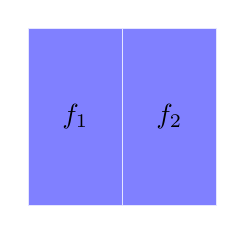
\begin{tikzpicture}[node distance=0cm,outer sep = 0pt,  baseline=(current bounding box.center)]
\tikzstyle{box}=[draw=blue!10, fill=blue!50, minimum width=2em, 
    text centered, minimum height=1.5em]
    \node (f1) [box,minimum height=6.4em, minimum width=3.4em] {$f_1$};
    \node (f2) [box,anchor=west,minimum height=6.4em, minimum width=3.4em] at (f1.east) {$f_2$};
\end{tikzpicture}
\quad \simeq \quad
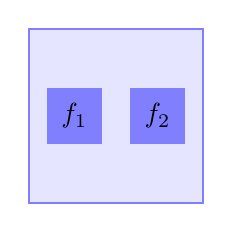
\begin{tikzpicture}[
    baseline=(current bounding box.center)
    ]
\tikzstyle{bigbox} = [draw=blue!50, thick, fill=blue!10, square]
\tikzstyle{box} = [square, draw=blue!10, fill=blue!50]
%
\matrix[row sep=2mm, column sep=3mm, inner sep=2mm, bigbox, every node/.style=box] {
\node {$f_1$}; & \node {$f_2$};\\
};
%
\end{tikzpicture}
\quad \simeq \quad
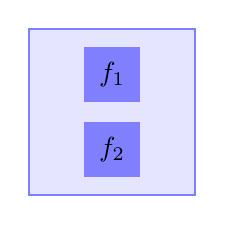
\begin{tikzpicture}[
    baseline=(current bounding box.center)
    ]
\tikzstyle{bigbox} = [draw=blue!50, thick, fill=blue!10, square]
\tikzstyle{box} = [square, draw=blue!10, fill=blue!50]
%
\matrix[row sep=2mm, column sep=3mm, inner sep=2mm, bigbox, every node/.style=box] {
\node {$f_1$};\\
\node {$f_2$};\\
};
%
\end{tikzpicture}
\quad \simeq \quad
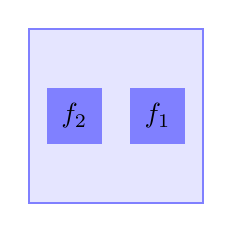
\begin{tikzpicture}[
    baseline=(current bounding box.center)
    ]
\tikzstyle{bigbox} = [draw=blue!50, thick, fill=blue!10, square]
\tikzstyle{box} = [square, draw=blue!10, fill=blue!50]
%
\matrix[row sep=2mm, column sep=3mm, inner sep=2mm, bigbox, every node/.style=box] {
\node {$f_2$}; & \node {$f_1$};\\
};
%
\end{tikzpicture}
\quad \simeq \quad
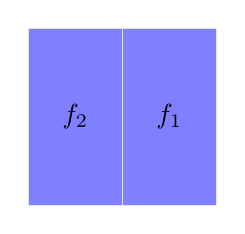
\begin{tikzpicture}[node distance=0cm,outer sep = 0pt,  baseline=(current bounding box.center)]
\tikzstyle{box}=[draw=blue!10, fill=blue!50, minimum width=2em, 
    text centered, minimum height=1.5em]
    \node (f1) [box,minimum height=6.4em, minimum width=3.4em] {$f_2$};
    \node (f2) [box,anchor=west,minimum height=6.4em, minimum width=3.4em] at (f1.east) {$f_1$};
\end{tikzpicture}
\]

\end{proof}


\begin{remark}
A map $f: S^{n-1} \to X$ is homotopic to the constant map if and only if there is some $g$ such that 
\[
\begin{tikzcd}
D^n \arrow[rd, "g"]                     &   \\
S^{n-1} \arrow[r, "f"'] \arrow[u, hook] & X
\end{tikzcd}
\] commutes.
\end{remark}

\begin{theorem}[Whitehead]\label{WH}
If $\psi: X \to Y$ is a map of connected cell complexes, then $f$ is a homotopy equivalence if and only if $\psi_{\ast} : \pi_n(X,x) \to \pi_n(Y, y)$ is an isomorphism for each $n \in \N$.
\end{theorem}

A map $f : X \to Y$ of path connected spaces is a \textit{weak homotopy equivalence} if it induces an isomorphism $\pi_n(X) \to \pi_n(Y)$ for each $n\in \N$. Since any cell complex is locally path connected, it is connected if and only if it is path connected. Hence \cref{WH} says that $\psi$ is a homotopy equivalence if and only if it is a weak homotopy equivalence.

\subsection{Lecture 3}

\begin{defn}
If $x\in A \subset X$, then the \textit{$n$-th relative homotopy group $\pi_n(X, A, x)$} consists of all homotopy classes of maps $\left(D^n, S^{n-1}, x_0\right) \to \left(X, A, x\right)$. 
\end{defn}

We see that  $$M((D^n, S^{n-1}, x), (X, A, x_0)) \cong M((I^n, I^{n-1} \times \{1\}, \underbrace{\partial{I^n} \setminus \Int(I^{n-1} \times \{1\})}_{\partial_0{I^n}}), (X, A, x_0))$$ by considering the homeomorphism $\left(I^n/\partial_0{I^n}, \partial{I^n}/\partial_0{I^n}\right) \cong \left(D^n, S^{n-1}\right)$. Therefore, $\pi_n(X, A, x)$ can be viewed as consisting of all homotopy classes of maps $\left(I^n, \partial{I^n}, \partial_0{I^n}\right) \to \left(X, A, x\right)$.

\begin{defn}
In order to interpret an exact sequence involving objects in the category of pointed sets, we define the \textit{kernel of a function $f: \left(X,x\right) \to \left(Y,y\right)$ of pointed sets} as $\ker{f} \equiv f^{-1}(y)$.   
\end{defn}

\begin{prop} $ $
\be
\item If $n\geq 2$, then $\pi_n(X, A, x)$ is, in fact, a group.
\item If $n\geq 3$, then $\pi_n(X, A, x)$ is abelian.
\item We have a long exact sequence 
\[
\begin{tikzcd}
\cdots \arrow[r] & {\pi_n(A,x)} \arrow[r]     & {\pi_n(X, x)} \arrow[r] & {\pi_n(X, A, x)} \arrow[r, "\partial"] & {\pi_{n-1}(A,x)} \arrow[llld] &   \\
                 & {\pi_{n-1}(X,x)} \arrow[r] & \cdots \arrow[r]        & {\pi_0(A, x)} \arrow[r]                & {\pi_0(X,x)} \arrow[r]        & 0
\end{tikzcd}
\] with $\partial{[f]} = \left[f\restriction_{I^{n-1}}\right]$.
\ee 
\end{prop}

\begin{theorem}[Hurewicz] 
Let $n\in \Z_{\geq 2}$. If $\pi_i(X) =0$ for each $i < n$, then $\pi_n(X) \cong H_n(X)$. 
\end{theorem}

\begin{note}
This result can't be improved in general. For example, $\pi_3(S^2) \cong \Z$, whereas $H_3(S^2) =0$.
\end{note}

Let $A \subset X$ be a subcomplex. Recall that $H_i(X, A) \cong H_i(X/A. \ast)$ for each $i\geq 1$. But it is \emph{not} the case that $\pi_i(X, A) \cong \pi_i(X/A. \ast)$, for otherwise  $\pi_i(S^n) \cong \pi_i(D^n, S^{n-1}) \cong \pi_i(S^{n-1})$, which is known to be false exactly when $i > 2n-2$. 

\begin{exmp}
$\pi_4(S^3) \cong \Z_2 \not \cong  \pi_4(S^4)$.
\end{exmp}

\bigskip

Finally, let's review the notion of a fibration of spaces.

\medskip

Consider any map $f: Z \to B$. Recall that if $p: E \to B$ is a covering projection, then TFAE.
\be
\item There exists a unique $\hat{f} : Z \to E$ such that $p \circ \hat{f} = f$.
\item $f_{\ast}(\pi_1(Z)) \subset p_{\ast}(\pi_1(E))$.
\ee

The existence of $\hat{f}$ follows from the fact that any covering space satisfies the homotopy lifting property.

\begin{defn}[Fibration]
Suppose that $p: E \to B$ is any map. We say that $p$ is a \textit{(Serre) fibration} if it satisfies the homotopy lifting property, i.e., given a commutative square
\[
\begin{tikzcd}
X\times \left\{0\right\} \arrow[d, hook] \arrow[r, "\widehat{f_0}"] & E \arrow[d, "p"] \\
{X\times \left[0,1\right]} \arrow[r, "f"']                      & B               
\end{tikzcd}
,\]  where $X$ is a cell complex, there is some $G$ such that
\[
\begin{tikzcd}
X\times \left\{0\right\} \arrow[d, hook] \arrow[r, "\widehat{f_0}"] & E \arrow[d, "p"] \\
{X\times \left[0,1\right]} \arrow[r, "f"'] \arrow[ru, "G"]      & B               
\end{tikzcd}
\] commutes. 
\end{defn}

\begin{theorem}
If $p: E \to B$ is a fibration with $e \in F \coloneqq p^{-1}(b)$, then $$p_{\ast} : \pi_i(E, F, e) \overset{\cong}{\longrightarrow} \pi_i(B, b, b) = \pi_i(B, b).$$
\end{theorem}
\begin{proof}
Let $f: \left(I^n, \partial{I^n}\right) \to \left(B, b\right)$. To prove that $p_{\ast}$ is surjective, it suffices to find some $G : \left(I^n, \partial{I^n}\right) \to \left(E, F\right)$ such that 
\[
\begin{tikzcd}
\partial_0{I^n} \arrow[r, two heads] \arrow[d, hook]       & \left\{e\right\} \arrow[r, hook] & F \arrow[r, hook] & E \arrow[d, "p"] \\
{I^{n-1} \times \left[0,1\right]} \arrow[rrr, "f"'] \arrow[rrru, "G"] &                       &                   & B               
\end{tikzcd}
\] commutes, for in this case $\left[p \circ G'\right] = \left[f\right]$. Since $p$ is a fibration, there is some $G$ such that
\[
\begin{tikzcd}
I^{n-1} \times \left\{0\right\} \arrow[r, two heads] \arrow[d, hook]       & \left\{e\right\} \arrow[r, hook] & F \arrow[r, hook] & E \arrow[d, "p"] \\
{I^{n-1} \times \left[0,1\right]} \arrow[rrr, "f"'] \arrow[rrru, "G'"] &                       &                   & B               
\end{tikzcd}
\] 
commutes. But $\left(I^n, \partial_0{I^n}\right) \cong \left(I^n, I^{n-1} \times \left\{0\right\}\right)$, and thus such a $G'$ is enough. 
\end{proof}

\begin{corollary}\label{exhtpy}
We have a long exact sequence 
\[
\begin{tikzcd}
\cdots \arrow[r] & {\pi_i(F, e)} \arrow[r] & {\pi_i(E, e)} \arrow[r] & {\pi_i(B, b)} \arrow[r, "\partial"] & {\pi_{i-1}(F, e)} \arrow[r] & \cdots
\end{tikzcd}
.\]
\end{corollary}

\begin{exmp} $ $
\be
\item Suppose that
\[
\begin{tikzcd}
X\times \left\{0\right\} \arrow[d, hook] \arrow[r, "\hat{f}"] & B \times F \arrow[d, "\pi_B"] \\
{X\times \left[0,1\right]} \arrow[r, "f"]                           & B                            
\end{tikzcd}
\] commutes. Then $\hat{f}(x,0) = \left(\hat{f}_1(x,0), \hat{f}_2(x,0)\right)$ where $\hat{f}_1(x,0) = f(x,0)$. Let $G(X,t) =  \left(f(x,t), \hat{f}_2(x,0)\right)$. Then \[
\begin{tikzcd}
X\times \left\{0\right\} \arrow[d, hook] \arrow[r, "\widehat{f_0}"] & B \times F \arrow[d, "\pi_B"] \\
{X\times \left[0,1\right]} \arrow[r, "f"] \arrow[ru, "G"]           & B                            
\end{tikzcd}
\] commutes, so that $\pi_B$ is a fibration. (Moreover, $\pi_n(B \times F) \cong \pi_n(B) \times \pi_n(F)$.)
\item Let $A \subset X$ be a subcomplex. The map $\varphi : M(X, Y) \to M(A, Y)$ defined by $f \mapsto f\restriction_A$ is a fibration. 
\item Define the \textit{Hopf fibration} as the quotient map
\[
S^3 = \left\{\left(z_1, z_2\right) \in \C^2 \mid z_1\overline{z_1} + z_2\overline{z_2} =1\right\} \twoheadrightarrow \faktor{S^3}{x \sim {-}x} = \CP^1 =S^2.
\]
\ee
\end{exmp}

\pagebreak

\begin{corollary}
$\pi_3(S^3) \cong \pi_3(S^2)$.
\end{corollary}
\begin{proof}
Since we have an exact sequence 
\[
\begin{tikzcd}
\pi_3(S^1) \arrow[r] & \pi_3(S^3) \arrow[r] & \pi_3(S^2) \arrow[r] & \pi_2(S^1)
\end{tikzcd},
\] it suffices to show that both $\pi_3(S^1)$ and $\pi_2(S^1)$ are trivial. To this end, note that since $\pi_1(S^k) =0$ for every $k>1$, we can always find,  for any $f: S^k \to S^1$,  a map $\hat{f}$ such that
\[
\begin{tikzcd}
                                                  & \R \arrow[d, "e^{2\pi i x}"] \\
S^k \arrow[r, "f"'] \arrow[ru, "\hat{f}"] & S^1                         
\end{tikzcd}
\] commutes. Thus, $f$ is homotopic to the constant map. Since $f$ was arbitrary, our proof is complete.
\end{proof}

\begin{defn}\label{ltriv}
A map $p : E \to B$ is \textit{locally trivial} if for any $b\in B$, there exist a neighborhood $U\ni b$ in $B$, a space $F$, and a homeomorphism $\varphi: p^{-1}(U) \overset{\cong}{\longrightarrow} U \times F$ such that $\pi_U \circ \varphi = p \restriction_{p^{-1}(U)}$.
\end{defn}

\begin{theorem}
Any locally trivial map $p: E \to B$ is a fibration whenever $B$ is a cell complex. 
\end{theorem}

\begin{exercise}
Prove that the Hopf fibration is locally trivial.
\end{exercise}
\begin{proof}
For each $k \in \{0,1\}$, let $U_k = \left\{\left[z_0, z_1\right] \in \CP^1 \mid z_k \ne 0\right\}$. Then $U_0$ and $U_1$ form an open cover of $\CP^1$. Note that the preimage of $U_k$ under the Hopf fibration $q$ is precisely $\left\{\left(z_0, z_1\right) \in S^3 \mid z_k \ne 0\right\}$. Define $f: q^{-1}(U_k) \to  U_k \times S^1$ by  $$\left(z_0, z_1\right) \mapsto \left(\left[z_0, z_1\right], \frac{z_k}{\left\lvert{z_k}\right\lvert}\right).$$ This is clearly continuous. Further, define the map $g: U_k \times S^1 \to q^{-1}(U_k)$ by $$\left(\left[z_0, z_1\right], e^{i{\theta}}\right) \mapsto \frac{e^{i\theta}\left\lvert{z_k}\right\rvert}{z_k \left\lvert{\left(z_0, z_1\right)}\right\rvert}\left(z_0, z_1 \right).$$ Since $U_k$ is a saturated open set, we have that the restriction of $q$ to $q^{-1}(U_k)$ is a quotient map. But $g \circ q\restriction_{q^{-1}(U_k)}$ is continuous, so that $g$ is also continuous by the characteristic property of quotient maps. Finally, it is easy to verify that $g$ and $f$ are inverses of each other and that $\pi_{U_I} \circ f = p\restriction_{q^{-1}(U_k)}$.
\end{proof}

\subsection{Lecture 4}

\begin{theorem}
Let $A\subset X$ be a subcomplex. Define $r: M(X, Y) \to M(A, Y)$ by $r(f) = f\restriction_A$. Then $r$ is a fibration. 
\end{theorem}
\begin{proof}
We must fill any diagram of the form
\[
\begin{tikzcd}
Z\times \left\{0\right\} \arrow[r, "\hat{f}"] \arrow[d, hook]                 & {M(X,Y)} \arrow[d, "r"] \\
{Z\times \left[0,1\right]} \arrow[ru, "F", dashed] \arrow[r, "f"'] & {M(A,Y)}               
\end{tikzcd}
.\] It suffices to find a map $\overline{F}$ such that
\[
\begin{tikzcd}
Z\times \left\{0\right\}\times X \arrow[r, "\hat{\bar{f}}"] \arrow[d, hook] & Y \arrow[d, equals] \\
{Z\times \left[0,1\right]\times X} \arrow[ru, "\overline{F}"]               & Y           \\
{Z\times \left[0,1\right]\times A} \arrow[u, hook] \arrow[ru, "\bar{f}"']   &            
\end{tikzcd}
\] commutes for, in this case, we can set $F(z,t)(x) = \overline{F}(z, t, x)$.

\begin{note}
Suppose that such an $\overline{F}$ exists. Define $g: Z \times X \to Y$ by $g(z,x) = \hat{\bar{f}}(z,0, x)$. Define $h: Z \times X \times \left[0,1\right] \to Y$ by $H(z,x,t) = \overline{F}(z,t,x)$. Then
\[
\begin{tikzcd}
Z\times X\times \left\{0\right\} \arrow[rd, "g"] \arrow[d, hook]     &   \\
{Z\times X \times \left[0,1\right]} \arrow[r, "H"]                   & Y \\
{Z\times A \times \left[0,1\right]} \arrow[u, hook] \arrow[ru, "K"'] &  
\end{tikzcd}
\]
commutes where $K(z,a,t) = \bar{f}(z,t,a)$. In the case where $Z = \pt$, this means that if $K: A \times \left[0,1\right] \to Y$ is a homotopy from a map $f: A \to Y$ and $g$ extends $f$ to $X$, then there exists a homotopy $H : X \times \left[0,1\right]\to Y$ such that $H\restriction_{A \times \left[0,1\right]} = K$. In other words, the extension problem for cell complexes is a homotopy problem. 
\end{note}
Let's return to proving our theorem. By induction, it suffices to consider just the case where $X = A \cup_{\varphi} D^n$, with characteristic map $\chi: D^n \to X$.   Thus, it suffices to find a map $w$ such that
\[
\begin{tikzcd}[column sep = huge]
Z\times D^n \times \left\{0\right\} \arrow[d, hook] \arrow[rrd, "\id_Z \times (g \circ \chi)"]                    &                                          &   \\
{Z\times D^n \times \left[0,1\right]} \arrow[rr, "w"]                                                                  &                                          & Y \\
{Z\times S^{n-1} \times \left[0,1\right]} \arrow[u, hook] \arrow[r, "{\id_Z \times \varphi \times \id_{\left[0,1\right]}}"'] & {Z\times A\times \left[0,1\right]} \arrow[ru, "K"'] &  
\end{tikzcd}
\] commutes for, in this case, we can set $H(z, x, t) = g \cup_{\varphi} w$, thereby making
\[
\begin{tikzcd}[column sep = huge]
Z\times D^n \times \left\{0\right\} \arrow[d, hook] \arrow[rrd, "\id_Z \times (g \circ \chi)"]                          &                                           &   \\
{Z\times D^n \times \left[0,1\right]} \arrow[r, "{\id_Z \times \chi \times \id_{\left[0,1\right]}}"'] \arrow[rr, "w"', bend right] & {Z\times X\times \left[0,1\right]} \arrow[r, "H"']   & Y \\
{Z\times S^{n-1} \times \left[0,1\right]} \arrow[u, hook] \arrow[rd, "{\id_Z \times \varphi \times \id_{\left[0,1\right]}}"']      &                                           &   \\
                                                                                                             & {Z\times A\times \left[0,1\right]} \arrow[ruu, "K"'] &  
\end{tikzcd}
\] commute. To this end, define the retraction $u : D^n \times \left[0,1\right] \to D^n \times \left\{0\right\} \cup S^{n-1} \times \left[0,1\right]$ by  picking a point $\ast$ directly above the cylinder $D^n \times \left[0,1\right]$ and then sending any point $x$ in the cylinder to the unique point where $D^n \times \left\{0\right\} \cup S^{n-1} \times \left[0,1\right]$ intersects the line containing $\ast$ and $x$. Now, define $w$ so that
\[
\begin{tikzcd}[column sep = huge]
{Z \times (D^n \times \left[0,1\right])} \arrow[d, "\id_Z \times u"'] \arrow[r, "w"]                                                                     & Y \\
{Z \times (D^n \times \left\{0\right\} \cup S^{n-1} \times \left[0,1\right])} \arrow[ru, "{\id_Z \times \left(g \circ \chi \cup K \circ (\varphi \times \id_{\left[0,1\right]})\right)}"'] &  
\end{tikzcd}
\] commutes. 
\end{proof}

\begin{exercise}\label{loop}
Let $x\in X$. Consider the  loop space $\Omega(X, x) \equiv M((S^1, \pt), (X, x))$. Prove that $\pi_n(\Omega{X})\cong \pi_{n+1}(X)$.
\end{exercise}
\begin{proof}
Consider the \textit{path space $P{X} \equiv \left\{\gamma : \left[0,1\right] \to X \mid \gamma(0) =x\right\}$ of $\left(X,x\right)$}, equipped with the compact-open topology. We claim that $P{X}$ is contractible. Indeed, define $K: P{X} \times \left[0,1\right] \to P{X}$ by $$\left(\gamma, t\right) \mapsto \left(s \mapsto \gamma(s(1-t))\right).$$ Then $K$ is a homotopy from $\id_{P{X}}$ to the constant map at the constant path at $x$.

\medskip

Define the map $p : P{X} \to X$ by $\gamma \mapsto \gamma(1)$. Then $p^{-1}(x) = \Omega(X)$. By \cref{exhtpy}, it suffices to show that $p$ is a fibration. To this end, suppose that the square
\[
\begin{tikzcd}
Y\times \left\{0\right\} \arrow[d, hook] \arrow[r, "\hat{f}"] & P{X} \arrow[d, "p"] \\
{Y\times \left[0,1\right]} \arrow[r, "f"']                    & X                  
\end{tikzcd}
\] commutes. Define $H: Y \times \left[0,1\right] \to P{X}$ by $\left(y, t\right) \mapsto  H(y,t)$ where 
\[
H(y, t)(s) = \begin{cases} 
\hat{f}(y)\left((1+t)s\right) & 0\leq s\leq \frac{1}{1+t}
\\ f(y, (1+t)s -1) & \frac{1}{1+t}\leq s \leq 1
\end{cases}.
\] We see that $H$ is continuous when viewed as a function of $\left(y,t,s\right)$ and thus is continuous. It is easy to check that 
\[
\begin{tikzcd}
Y\times \left\{0\right\} \arrow[d, hook] \arrow[r, "\hat{f}"] & P{X} \arrow[d, "p"] \\
{Y\times \left[0,1\right]} \arrow[r, "f"'] \arrow[ru, "H"]    & X                  
\end{tikzcd}
\] commutes, as desired.
\end{proof}

Let $p : E \to B$ be a map. Recall that the pullback of $p$ along $f : X \to B$ is given explicitly as   $$f^{\ast}{E} \equiv \left\{\left(x, e\right) \in X \times E \mid f(x) = p(e)\right\}.$$  Let  $f^{\ast}{p}$ denote the map $\pi_X\restriction_{f^{\ast}{E}}$.

\begin{prop}
If $p$ is a fibration, then so is $f^{\ast}{p}$.
\end{prop}

\begin{lemma}\label{pbtriv}
If $p$ is locally trivial, then so is $f^{\ast}{p}$. 
\end{lemma}
\begin{proof}
Let $a \in X$. Since $p$ is locally trivial by assumption, we can find a neighborhood $U$ of $f(a)$ in $B$ and a homeomorphism $\varphi : p^{-1}(U) \to U \times F$. Observe that 
\[
(f^{\ast}{p})^{-1}(f^{-1}(U)) = \left\{\left(x,e\right) \mid f(x) = p(e), \ f(x) \in U\right\} \subset f^{-1}(U) \times p^{-1}(U).
\] Further, we have a map $\psi : f^{-1}(U) \to p^{-1}(U) \to f^{-1}(U) \times F$ given by $\left(x,e\right) \mapsto \left(x, \pi_F(\varphi(e))\right)$. Define $\lambda : f^{-1}(U) \times F \to (f^{\ast}{p})^{-1}(f^{-1}(U))$ by $\left(x,y\right) \mapsto \left(x, \varphi^{-1}(f(x), y)\right)$. Using the fact that 
\[
\begin{tikzcd}
p^{-1}(U) \arrow[r, "\varphi"] \arrow[rd, "p"'] & U\times F \arrow[d, "\pi_U"] \\
                                                    & U                           
\end{tikzcd}
\] commutes, it is easy to check that $\psi$ and $\lambda$ are inverses of each other. 
\end{proof}



\subsection{Lecture 5}

\begin{theorem}
Let $B$ be a cell complex and let $p : E \to B$ be locally trivial. Then $p$ is a fibration. 
\end{theorem}
\begin{proof}
It suffices to prove the following claim: 
\begin{addmargin}[1em]{2em}

\smallskip

If $h : Z \to X \times \left[0,1\right]$ is locally trivial, $X = \bigcup_{i=0}^n X^i$ is a cell complex, and $\sigma_0 : X \times \left\{0\right\} \to Z$ satisfies $h \circ \sigma_0 = \id_{X \times \left\{0\right\}}$, then there is some map $\sigma : X \times \left[0,1\right] \to Z$ such that $\sigma_{X \times \left\{0\right\}} = \sigma_0$ and $h \circ \sigma = \id_{X \times \left[0,1\right]}$.
\end{addmargin}

\smallskip

For, in this case, \cref{pbtriv} implies that given any commutative square
\[
\begin{tikzcd}
X \times \left\{0\right\} \arrow[d, hook] \arrow[r, "\hat{f}"] & E \arrow[d, "p"] \\
{X \times \left[0,1\right]} \arrow[r, "f"']                    & B               
\end{tikzcd}
,\] we can find some $\sigma$ such that
\[
\begin{tikzcd}
                                                      & f^{\ast}{E} \arrow[r] \arrow[d]                                   & E \arrow[d, "p"] \\
X \times \left\{0\right\} \arrow[ru, "\sigma_0"] \arrow[r, hook] & {X \times \left[0,1\right]} \arrow[r, "f"'] \arrow[u, "\sigma"', bend right] & B               
\end{tikzcd}
\] commutes where $\sigma_0(x,0) = \left(x,0, \hat{f}(x,0)\right)$.

\medskip

For induction, let us assume that our claim is true for each $X^0, X^1, \ldots, X^{n-1}$. We may assume, wlog, that $X = D^n$. It suffices to find a map $\tau : S^{n-1} \times \left[0,1\right] \to Z$ such that $h \circ \tau = \id_{S^{n-1}\times \left[0,1\right]}$ and
\[
\begin{tikzcd}
                                                        & Z \arrow[d, "h"]                                       &                                                           \\
D^n \times \left\{0\right\} \arrow[r, hook] \arrow[ru, "\sigma_0"] & {D^n \times \left[0,1\right]}                                     & {S^{n-1}\times \left[0,1\right]} \arrow[l, hook] \arrow[lu, "\tau"', dashed] \\
                                                        & S^{n-1} \times \left\{0\right\} \arrow[lu, hook] \arrow[ru, hook] &                                                          
\end{tikzcd}
\] commutes as there is a retraction $$r: D^n \times \left[0,1\right] \to D^{n} \times \left\{0\right\} \cup S^{n-1}\times \left[0,1\right].$$ To this end, fix a positive integer $m$. For each $j\in \left\{0,1, \ldots, m\right\}$, let $a_j = \frac{j}{m}$ and let $I_j = \left[a_j, a_{j+1}\right]$. Since $D^n \times \left[0,1\right]$ is compact,  by making $m$ large enough, we can ensure that $h\restriction_{h^{-1}(I_{j_1} \times \cdots \times I_{j_{n+1}})}$ is trivial.
\begin{claim}
$h\restriction_{h^{-1}(I_{j_1} \times \cdots \times I_{j_n} \times  \left[0,1\right])}$ is also trivial. 
\end{claim}
\begin{proof}
We may assume, wlog, that $h$ is trivial on $h^{-1}(I_{j_1} \times \cdots \times I_{j_n} \times  I_j)$ for any $j$. Let $k\in \left\{0, 1, \ldots, m-1\right\}$ and assume, for induction, that $h$ is trivial on $h^{-1}(I_{j_1} \times \cdots \times I_{j_n} \times  \left[0,a_k\right])$. Let $K = I_{j_1} \times \cdots \times I_{j_n}$ and $J = K\times \left[0, a_k\right]$ and $\tilde{J}= K\times \left[a_k, a_{k+1}\right]$. By assumption, there exists a homeomorphism $\varphi :h^{-1}(J) \overset{\cong}{\longrightarrow} J\times F$ such that $\pi_J \circ \varphi =h$. Likewise, there exists a homeomorphism $\psi : h^{-1}(\tilde{J}) \overset{\cong}{\longrightarrow} \tilde{J} \times F$ such that $\pi_{\tilde{J}} \circ \psi = h$.

\smallskip

If $\psi =\varphi$ on $K\times \left\{a_k\right\}$, then $h^{-1}(J\cup \tilde{J}) \overset{\varphi \cup \psi}{\longrightarrow} \left(J \cup \tilde{J}\right) \times F$ is a well-defined trivialization, in which case we're done. With this in mind, let
\[
w = \left(\varphi\restriction_{K\times \left\{a_k\right\}} \circ \left(\psi\restriction_{K\times \left\{a_k\right\}}\right)^{-1}\right) \times \id_{\left[a_k, a_{k+1}\right]}
.\]
Note that 
\[
\begin{tikzcd}
h^{-1}(\tilde{J}) \arrow[r, "\psi"] \arrow[d, "h"'] & \tilde{J}\times F \arrow[d, "w \times \id_F"]               \\
\tilde{J}                                           & \tilde{J}\times F \arrow[l, "\pi_{\tilde{J}}"]
\end{tikzcd}
\] commutes and that $\gamma \coloneqq \left(\left(w \times \id_F\right) \circ \psi\right)$ agrees with $\varphi$ on $K\times \left\{a_k\right\}$. Hence we may take $\varphi \cup \gamma$ as our desired trivialization.
\end{proof}
As a result, we may assume that $h$ is trivial on its entire domain, i.e., that $h$ is the projection $$\left(D^n \times \left[0,1\right]\right) \times F \twoheadrightarrow D^n \times \left[0,1\right].$$ Moreover, by induction, we can find a right inverse $\sigma : X^{n-1} \times \left[0,1\right] \to D^n \times \left[0,1\right]$ of $h : Z \to X^{n-1} \times \left[0,1\right]$ that extends $\sigma_0\restriction_{X^{n-1}\times \left\{0\right\}}$. But $X^{n-1}$ consists of all $\left(n-1\right)$-dimensional faces of the $n$-cube, and thus we have a map $$\tau \equiv \sigma \restriction_{\partial{I^n} \times \left[0,1\right]} : S^{n-1} \times  \left[0,1\right]   \to  \left(D^n \times \left[0,1\right]\right) \times F,$$ which has the form $\left(x,t\right) \mapsto \left(x,t,\tilde{\tau}(x,t)\right)$. Further, $\sigma_0$ has the form $\left(x,0\right) \mapsto \left(x,0, \tilde{\sigma}_0(x,0)\right)$. Therefore, our desired map $\sigma :  D^n \times \left[0,1\right] \to \left(D^n \times \left[0,1\right]\right) \times F $  is given by 
\[
\sigma(x,t) = \left(x,t, \left(\tilde{\sigma}_0 \cup \tilde{\tau}\right)(r(x,t))\right).
\]
\end{proof}


\section{Fiber bundles}

\begin{defn}
A \textit{topological group} $G$ is a group such that both multiplication $G \times G \overset{\mu}{\longrightarrow} G$ and inversion $G \overset{{-}^{-1}}{\longrightarrow} G$ are continuous.
\end{defn}

\begin{defn}[Fiber bundle] Let $G$ be a topological group.
\be 
\item A \textit{fiber $F$ of $G$} is a space equipped with a faithful (i.e., injective) group action $\rho : G \to \homeo(F) \subset M(F, F)$. 
\item An \textit{atlas for the structure of a (fiber) bundle with group $G$ and fiber $F$ on a map $p: E \to B$} consists of 
\be
\item a family $\left(U_{\alpha}, h_{\alpha}\right)_{\alpha \in A}$ where each $U_{\alpha}$ is open and each $h_{\alpha}$ is a homeomorphism $p^{-1}(U_{\alpha}) \to U_{\alpha} \times F$ and
\item  a family of continuous \textit{transition functions} $\left\{h_{\beta{\alpha}} : U_{\alpha} \cap U_{\beta} \to G\right\}_{\alpha, \beta \in A}$ 
\ee such that
\be[label= \roman*]
\item $B = \bigcup_{\alpha \in A} U_{\alpha}$,
\item $\pi_{U_{\alpha}} \circ h_{\alpha} = p\restriction_{p^{-1}(U_{\alpha})}$, and
\item  $x\in U_{\alpha} \cap U_{\beta} \implies h_{\beta} \circ h_{\alpha}^{-1}(x,f) = \left(x, h_{\beta{\alpha}}(x)\cdot f\right)$
\ee
\item Two atlases are \textit{compatible} if their union is an atlas. 
\item A \textit{bundle structure on $B$} is a maximal atlas on $p$. 
\ee
\end{defn}

\begin{term}
If $B$ is equipped with a bundle structure, then we say that $p$ is a (fiber) bundle.
\end{term}

\begin{exmp} $ $
\be
\item The tangent bundle $\pi : TM \to M$ of a smooth $n$-manifold $M$ is a bundle with group $\GL(n, \R)$.
\begin{proof}
Let $\left(U, \varphi\right)$ be any coordinate chart for $M$ with coordinate functions $\left(x^i\right)$. Define $h: \pi^{-1}(U) \to U \times \R^n$ by $$v^i\frac{\partial}{\partial{x^i}}\left(p\right) \mapsto \left(p, \left(v^1, \ldots, v^n\right)\right).$$ It is clear that $\pi_{U}(h(p)) = \pi(c)$ for any $c\in \pi^{-1}(U)$. To see that $h$ is a homeomorphism, note that the composite $\left(\varphi \times \id_{\R^n}\right) \circ h : \pi^{-1}(U) \to \varphi(U) \times \R^n$ is given by $$v^i\frac{\partial}{\partial{x^i}}\left(p\right) \mapsto \left(x^1(p), \ldots, x^n(p), v^1, \ldots, v^n\right),$$ the inverse of which is given by $\left(x^1, \ldots, x^n, v^1, \ldots, v^n\right) \mapsto v^i\frac{\partial}{\partial{x^i}}\left(\varphi^{-1}(x)\right)$. Therefore,  $\left(\varphi \times \id_{\R^n}\right) \circ h$ is given locally by 
\[
\left(x^1, \ldots, x^n, v^1, \ldots, v^n\right) \mapsto \left(\tilde{x}^1(x), \ldots, \tilde{x}^n(x), \frac{\partial{\tilde{x}^1}}{\partial{x^j}}(x)v^j, \ldots, \frac{\partial{\tilde{x}^n}}{\partial{x^j}}(x)v^j\right),
\] which is smooth. Thus, $h$ is a diffeomorphism as the composite of two diffeomorphisms. In particular, $h$ is a homeomorphism. 

\smallskip

It remains to describe the transition functions $\left\{h_{\beta{\alpha}} : U_{\alpha} \cap U_{\beta} \to \GL(n, \R)\right\}$ for $T{M}$. Note that 
\[
\begin{tikzcd}
U_{\alpha{\beta}}\times \R^n \arrow[rd, "\pi_1"'] & \pi^{-1}(U_{\alpha{\beta}}) \arrow[l, "h_{\alpha}"'] \arrow[r, "h_{\beta}"] \arrow[d, "\pi"] & U_{\beta{\alpha}}\times \R^n \arrow[ld, "\pi_1"] \\
                                                  & U_{\alpha{\beta}}                                                                              &                                                 
\end{tikzcd}
\] 
commutes. In particular, $\pi_1 \circ h_{\beta} \circ h_{\alpha}^{-1} = \pi_1$, which implies that $ h_{\beta} \circ h_{\alpha}^{-1}(u,v) =\left(u, f(u,v)\right) $ for some smooth map $f: U_{\alpha{\beta}} \times \R^n \to \R^n$. This must be a linear isomorphism when restricted to $\left\{u\right\}\times \R^n$ for any $u\in U_{\alpha{\beta}}$, which is uniquely determined by an element $h_{\beta{\alpha}}(u)$ of $\GL(n, \R)$ (provided that we have fixed a basis of $\R^n$). Hence $$ h_{\beta} \circ h_{\alpha}^{-1}(u,v) =\left(u, h_{\beta{\alpha}}(u) v\right) .$$ Since the map $h_{\beta{\alpha}} :U_{\alpha{\beta}} \to \GL(n, \R)$ is continuous, our proof is complete.
\end{proof}

\item Let $p: E \to B$ be any bundle with group $\left\{e\right\}$. Then $p$ is the trivial bundle, i.e., is isomorphic to the projection map. \begin{proof}
We have that $h_{\beta} = h_{\alpha}$ on $p^{-1}(U_{\alpha} \cap U_{\beta}) = p^{-1}(U_{\alpha})\cap p^{-1}(U_{\beta})$, so that $h \equiv \bigcup_{\alpha \in A}h_{\alpha}$ is a well-defined homeomorphism $E \cong B \times F$.
\end{proof}
\ee 
\end{exmp}

\subsection{Lecture 6}

Let $\left\{\left(U_{\alpha}, h_{\alpha}\right)\right\}$ be a bundle structure with group $G$ and fiber $F$ on $p: E \to B$. Let $U = U_{\alpha} \cap U_{\beta} \cap U_{\gamma}$. 
Consider the commutative diagram
\[
\begin{tikzcd}
                                                                           &                                     & p^{-1}(U) \arrow[rrd, "h_{\gamma}"]    &                                      &           \\
U\times F \arrow[r, "h_{\alpha}^{-1}"'] \arrow[rru, "h_{\alpha}^{-1}"] & p^{-1}(U) \arrow[r, "h_{\beta}"'] & U\times F \arrow[r, "h_{\beta}^{-1}"'] & p^{-1}(U) \arrow[r, "h_{\gamma}"'] & U\times F
\end{tikzcd}.
\]
The bottom row is given by $\left(u, f\right) \mapsto \left(u, h_{\beta{\alpha}}(u) \cdot f\right) \mapsto \left(u, h_{\gamma{\beta}}(u) \cdot  \left( h_{\beta{\alpha}}(u) \cdot f\right)\right) =   \left(u, \left( h_{\gamma{\beta}}(u)  h_{\beta{\alpha}}(u)\right) \cdot f\right)$, and the top composite is given by $\left(u, f\right) \mapsto \left(u, h_{\gamma{\alpha}}(u)\cdot f\right)$.
 It follows that $$h_{\gamma{\beta}}(u)  h_{\beta{\alpha}}(u) = h_{\gamma{\alpha}}(u)$$ for each $u\in U$. This property is known as the \textit{cocycle condition}.

\begin{theorem}
Let $G$ be a topological group acting on a space $F$. Suppose that $\left\{U_{\alpha}\right\}$ is an open cover of $B$ and $\left\{h_{\beta{\alpha}} : U_{\alpha}\cap U_{\beta} \to G\right\}$ is a family of continuous functions satisfying the cocycle condition. Then there exists a bundle $p: E \to B$ with group $G$, fiber $F$, and transition functions  $h_{\beta{\alpha}}$.
\end{theorem}
\begin{proof}[Proof sketch]
Let $E = \faktor{\coprod_{\alpha}{U_{\alpha} \times F}}{\sim}$ where $\left(u, f\right)_{\alpha} \sim \left(u, h_{\beta{\alpha}}
(u) \cdot f\right)_{\beta}$. Define $p: E \to B$ by $\left(u, f\right) \mapsto  u$.
\end{proof}

\begin{defn}[Bundle map]
A \textit{morphism of bundles $p_1$ and $p_2$ with group $G$ and fiber $F$} is a commutative square of the form
\[
\begin{tikzcd}
E_1 \arrow[r, "\hat{g}"] \arrow[d, "p_1"'] & E_2 \arrow[d, "p_2"] \\
B_1 \arrow[r, "g"']                        & B_2                 
\end{tikzcd}
.\]
\end{defn}

Suppose that $\left(\hat{g}, g\right)$ is a bundle map $p_1 \to p_2$.  Let $\left\{\left(U_{\alpha}, h_{\alpha}\right)\right\}$ and $\left\{\left(V_{\beta}, k_{\beta}\right)\right\}$ be bundle structures on $B_2$ and $B_1$, respectively.  We have a commutative diagram
\[
\begin{tikzcd}
\left(g^{-1}(U_{\alpha}) \cap V_{\beta}\right) \times F \arrow[rd, "\pi_1"'] \arrow[rrr, "d_{\alpha{\beta}}", bend left] \arrow[r, "k_{\beta}^{-1}"] & p^{-1}_1\left(g^{-1}(U_{\alpha}) \cap V_{\beta}\right) \arrow[d] \arrow[r, "\hat{g}"] & p^{-1}_2(U_{\alpha}) \arrow[d] \arrow[r, "h_{\alpha}"] & U_{\alpha}\times F \arrow[ld, "\pi_1"] \\
                                                                                                                                                         & g^{-1}(U_{\alpha})\cap V_{\beta} \arrow[r, "g"']                                        & U_{\alpha}                                               &                                       
\end{tikzcd}
,\] so that $d_{\alpha{\beta}}(x,f)  = \left(g(x), \lambda_{\alpha{\beta}}(x) \cdot f\right)$ for some continuous map $\lambda_{\alpha{\beta}} : g^{-1}(U_{\alpha})\cap V_{\beta} \to G$. Letting $W = g^{-1}(U_{\alpha} \cap U_{\alpha'}) \cap (V_{\beta} \cap V_{\beta'})$, we have that 
\[
h_{\alpha'{\alpha}}(w)\lambda_{\alpha{\beta}}(w)k_{\beta{\beta'}}(w) = \lambda_{\alpha'{\beta'}}(w) \label{eq:mapcycle} \tag{$\dagger$}
\] for every $w\in W$.

\begin{exercise}[Pullback bundle]
Let  $\left\{\left(U_{\alpha}, h_{\alpha}\right)\right\}$ be a bundle structure on $p: E \to B$ with group $G$ and consider the pullback diagram \[
\begin{tikzcd}
g^{\ast}{E} \arrow[d, "g^{\ast}{p}"'] \arrow[r] & E \arrow[d, "p"] \\
X \arrow[r, "g"']                               & B               
\end{tikzcd}
.\] Define $h'_{\beta{\alpha}}: g^{-1}(U_{\alpha}) \cap g^{-1}(U_{\beta}) \to G$ as the composite $h_{\beta{\alpha}} \circ g$ restricted to  $g^{-1}(U_{\alpha} \cap U_{\beta})$. Show that the family $\left\{h'_{\beta{\alpha}}\right\}$ induces a bundle structure on $g^{\ast}{p}$.
\end{exercise}

\begin{theorem}\label{factors}
Every bundle map
\[
\begin{tikzcd}
E_1 \arrow[d, "p_1"'] \arrow[r, "\hat{g}"] & E_2 \arrow[d, "p_2"] \\
B_1 \arrow[r, "g"']                        & B_2                 
\end{tikzcd}
\]
factors as
\[
\begin{tikzcd}
E_1 \arrow[r, "\tau"] \arrow[d, "p_1"'] & g^{\ast}{E_2} \arrow[r, "\bar{g}"] \arrow[d, "g^{\ast}{p_2}"] & E_2 \arrow[d, "p_2"] \\
B_1 \arrow[r, "\id_{B_1}"']            & B_1 \arrow[r, "g"']                                           & B_2                 
\end{tikzcd}
\]
where $\tau(e) = \left(p_1(e), \hat{g}(e)\right)$ for any $e\in E_1$.
\end{theorem}

\subsection{Lecture 7}

\begin{note}\label{trnote}
If $\left\{h_{\beta{\alpha}}:U_{\alpha}\cap U_{\beta}\to G\right\}$ is a family of transition functions, then
\[
h_{\alpha{\beta}}(x) = \left(h_{\beta{\alpha}}(x)\right)^{-1}
\] for any $x\in U_{\alpha}\cap U_{\beta}$. In particular, $h_{\alpha{\alpha}}(x) = \left(h_{\alpha{\alpha}}(x)\right)^{-1}$.
\end{note}

\begin{theorem}
Any bundle map of the form
\[
\begin{tikzcd}
E_1 \arrow[rd, "p_1"'] \arrow[r, "\hat{g}"] & E_2 \arrow[d, "p_2"] \\
                                            & B                   
\end{tikzcd}
\]
is an isomorphism.
\end{theorem}
\begin{proof}
Note that
\[
\begin{tikzcd}
                                                         & p_2^{-1}(U_{\alpha}\cap U_{\beta}) \arrow[ld, "h_{\beta}"'] \arrow[rd, "h_{\alpha}"]      &                                                                                          \\
\left(U_{\alpha}\cap U_{\beta}\right)\times F \arrow[rd] & p_1^{-1}(U_{\alpha}\cap U_{\beta}) \arrow[u, "\hat{g}"] \arrow[d] \arrow[l, "k_{\beta}"'] & \left(U_{\alpha}\cap U_{\beta}\right)\times F \arrow[l, "k_{\alpha}^{-1}"'] \arrow[ld] \\
                                                         & U_{\alpha}\cap U_{\beta}                                                                    &                                                                                         
\end{tikzcd}
\] commutes.  We have that $h_{\beta} \circ \hat{g} \circ k_{\alpha}^{-1}(x,f) = \left(x, \lambda_{\beta{\alpha}}(x)\cdot f\right)$. Thus, if  $h_{\alpha}(e) = \left(x,f\right)$, then $h_{\alpha}\left(\hat{g}(e)\right) = \left(x, \lambda_{\alpha{\alpha}}(x) \cdot d\right).$ Let $$\left(\hat{g}\right)^{-1}(e) = k_{\alpha}^{-1}\left(x, \lambda_{\alpha{\alpha}}(x)^{-1}\cdot f\right)$$ where $\left(x,f\right) = h_{\alpha}(e)$. If this is well-defined on $E_2$ (??), then it indeed equals the inverse of $\hat{g}$.  Moreover, by \cref{trnote}, it is easy to check that $d_{\alpha'{\beta'}}(x)^{-1}$ satisfies \eqref{eq:mapcycle}, and thus it can be shown that $\left(\hat{g}\right)^{-1}$ is a bundle map.

\end{proof}

\begin{corollary}
Every bundle $E\to X$ is isomorphic to the pullback of $E$ by $\id_X$.
\end{corollary}

Let $\left\{\left(U_{\alpha}, h_{\alpha}\right)\right\}$ be a bundle structure with group $G$ and fiber $G$ on $p: E \to X$. In particular,
\[
\begin{tikzcd}
U_{\alpha}\times G \arrow[d, "\pi_1"'] & p^{-1}\left(U_{\alpha}\right) \arrow[l, "h_{\alpha}"'] \arrow[ld, "p"] \\
U_{\alpha}                             &                                                                                
\end{tikzcd}
\]
commutes. Define the free action $E \times G \to E$ by
\[
e\cdot g = h_{\alpha}^{-1}\left(h_{\alpha}(e)\cdot g\right).
\] where $p(e) \in U_{\alpha}$ and $\left(u,h\right) \cdot g \equiv \left(u, hg\right)$. This is well-defined because it does not depend on our choice of $\alpha$. Indeed, suppose that $p(e)$ also belongs to $U_{\beta}$. We have that $h_{\alpha}(e) =\left(p(e), h\right)$ and $h_{\beta}(e) = \left(p(e), h'\right)$ for some $h, h' \in G$. Then $e\cdot g = h_{\alpha}^{-1}\left(p(e), hg\right)$, and we must show that this equals $h_{\beta}^{-1}\left(p(e), h'g\right)$.  Note that $h_{\beta}\left(e\cdot g\right) = \left(p(e), h_{\beta{\alpha}}(p(e))hg\right)$.  But $$\left(p(e), h_{\beta{\alpha}}(p(e))h\right)  =  h_{\beta}\left(h_{\alpha}^{-1}\left(p(e), h\right)\right) = \left(p(e), h'\right),$$ 
so that $h_{\beta{\alpha}}(p(e))h = h'$, and thus $h_{\beta}\left(e\cdot g\right) = \left(p(e), h'g\right)$, as desired.

\begin{note}\label{quot}
$\faktor{E}{G} \cong \{p^{-1}(x) \mid x \in X \} \cong X$.
\end{note}

\begin{defn}[Balanced product]
Let $F$ be a space. The \textit{balanced product $E\times_G F$ of $E$ and $F$} is the quotient space $ \faktor{E\times F}{\sim}$ where $$\left(e, f\right)  \sim \left(eg, g^{-1}f\right)$$
for any $e\in E$ and $f\in F$.
\end{defn}

By the universal property of the quotient space, there is a unique map $\bar{p}$ such that
\[
\begin{tikzcd}
E\times F \arrow[d, "p\circ \pi_E"'] \arrow[r, two heads] & E\times_GF \arrow[ld, "\bar{p}"] \\
X                                                         &                                 
\end{tikzcd}. \label{eq:indmap}  \tag{$\star$}
\]

\begin{notation}
Let $\B\left(X, G, \rho, F\right)$ denote the set of all isomorphism classes of bundles over $X$ with group $G$ and fiber $F$. 
\end{notation}

\begin{lemma}
$\bar{p}$ is a bundle with group $G$ and fiber $F$.
\end{lemma}
\begin{proof}
As $\left(g,f\right)\sim \left(e_G, gf\right)$, we see that $\left( U \times G\right) \times_G F\cong U\times F$. Thus, we can endow $\bar{p}$ with local trivializations and transition functions that are exactly similar to those for $p$.
\end{proof}

\begin{prop}\label{iso}
 The function $p\mapsto \bar{p}$ defines a set isomorphism $\B\left(X, G, \rho, G\right) \overset{\cong}{\longrightarrow} \B\left(X, G, \rho, F\right)$. 
\end{prop}

Let $p_1 : E \to B_1$ and $p_2 : E \to B_2$ be bundles. Let $e_1 \in E_1$, $e_2\in E_2$, and $b_1\in B_1$.

\begin{question}
Can we find a bundle map
\[
\begin{tikzcd}
E_1 \arrow[r, dashed] \arrow[d, "p_1"'] & E_2 \arrow[d, "p_2"] \\
B_1 \arrow[r, dashed]                   & B_2                 
\end{tikzcd}
\]
such that $e_1\mapsto e_2$ and $e_1\mapsto b_1$?
\end{question}

Define the action $G\times E_2 \to E_2$ by $g\ast e_2 = e_2\cdot g^{-1}$. From this, we obtain a bundle $$\psi: \underbrace{E_1 \times_G E_2}_{\left(E_1 \times E_2\right)\mathbin{/}{G}} \to E_1 \times_G \pt \cong B_1$$ with fiber $E_2$.

\begin{lemma}\label{corr}
There is a one-to-one correspondence between bundle maps $p_1\to p_2$ and sections of $\psi$.
\end{lemma}
\begin{proof}
Suppose that $\sigma$ is a section of $\psi$.  As $G$ acts freely on $E_1 \times E_2$, we see that for any $e\in E_1$, there exists a unique $\tilde{e}$ such that $\sigma\left(p(e)\right)=\left[\left(e, \tilde{e}\right)\right]$. Define $\hat{g} : E_1\to E_2$ by $e\mapsto \tilde{e}$. This respects the action of $G$ and thus must be a bundle map.
\end{proof}

Now, let $A\subset B_1$ and suppose that
\[
\begin{tikzcd}
p_1^{-1}(A) \MySymb{dr} \arrow[r] \arrow[d] & E_2 \arrow[d, "p_2"] \\
A \arrow[r]                       & B_2                 
\end{tikzcd}
\]
is a bundle map.  Then $\alpha$ extends when {??}. Also, the corresponding section $$\sigma : A \to p^{{-1}}(A) \times_G E_2 \subset E_1 \times_G E_2$$ extends.

\begin{defn}[Principal bundle]
Let $G$ be a topological group. A \textit{principal $G$-bundle} is a fiber bundle with group $G$ and fiber $G$ with $G$ acting on itself by left translation.
\end{defn} 


\begin{theorem}\label{class}
Let $f$ and $g$ be homotopic maps $X \to Y$. Let $p: E \to Y$ be any bundle with group $G$ and fiber $F$. Then $f^{\ast}{p} \cong g^{\ast}{p}$.
\end{theorem}



\subsection{Lecture 8}

Before proving this, we wish to determine when, given any two bundles $p_1 : E_1 \to B_1$ and $p_2 : E_2 \to B_2$ and any map $g: B_1 \to B_2$, we can find a map $\hat{g}$ such that  
\[
\begin{tikzcd}
E_1 \arrow[d, "p_1"'] \arrow[r, "\hat{g}"] & E_2 \arrow[d, "p_2"] \\
B_1 \arrow[r, "g"']                        & B_2                 
\end{tikzcd}
\] commutes.

Define the \textit{diagonal action $\Delta{G}$} of $G$ on $E_1 \times E_2$ by $$\left(e_1, e_2\right)\cdot h = \left(e_1\cdot h, e_2 \cdot h\right),$$ so that $E_1 \times_G E_2 = \faktor{E_1 \times E_2}{\Delta{G}}$. By \eqref{eq:indmap}, we can find a unique map $\tau$ such that
\[
\begin{tikzcd}
E_1\times_G E_2 \arrow[rd, "\tau"] \arrow[d] &                                  \\
B_1                                          & B_1\times B_2 \arrow[l, "\pi_1"]
\end{tikzcd}
\] commutes.

\begin{exercise}
Show that $\hat{g}$ exists if and only if there is some $\lambda : B_1 \to E_1 \times_G E_2$ such that $\tau\left(\lambda\left(b_1\right)\right) = \left(b_1, g(b_1)\right)$.
\end{exercise}
\begin{proof} $ $ \\
$\left(\Longleftarrow\right)$ As $G$ acts freely on $E_1 \times E_2$, we see that $\left(e, e' \right) \sim \left(e, e''\right) \implies e'=e''$ for any $e', e'' \in E_2$. Hence for any $e \in E_1$, there exists a unique $\hat{e} \in E_2$ such that $\lambda\left(p_1(e)\right) = \left[\left(e, \hat{e}\right) \right]$. Let $\hat{g}(e) = \hat{e}$. Then $\hat{g}$  is clearly continuous and $G$-equivariant, and thus $\left(\hat{g}, g\right)$ is a bundle map.

\medskip

$\left(\Longrightarrow\right)$ Consider the homeomorphism $\varphi : B_1 \overset{\cong}{\longrightarrow} \faktor{E_1}{G}$ with $\varphi(b) = p_1^{-1}(b)$. Let $b\in B_1$. Let $\varphi(b) = \left[e\right]$. Define $\lambda : B_1 \to E_1 \times_G E_2$ by $\lambda(b) = \left[\left(e, \hat{g}(e)\right)\right]$. Since $\hat{g}$ is $G$-equivariant, we see that $\lambda$ is well-defined. Further, $\lambda$ is continuous as the quotient of the map 
\[ f : E_1 \to E_1 \times E_2, \quad f(x) = \left(x, \hat{g}(x)\right)
\] by $G$.  Finally, it is easy to check that $\tau\left(\lambda\left(b_1\right)\right) = \left(b_1, g(b_1)\right)$ for any $b_1 \in B_1$.
\end{proof}


\begin{lemma}\label{ttriv}
$\tau$ is locally trivial, hence a fibration.
\end{lemma}
\begin{proof}
Locally, we have that $E_1 \cong U \times G$ and $E_2 \cong V \times G$, so that $E_1 \times E_2 \cong U \times V \times G \times G$. It follows that, locally, $E_1\times_G E_2 \cong U_1  \times U_2 \times \faktor{G\times G}{\Delta{G}}$ where $\Delta{G} \equiv \{\left(g, g\right) \mid g\in G\}$.
\end{proof}

\begin{remark}
In fact, $\tau$ is a bundle with fiber $\faktor{G\times G}{\Delta{G}} \cong G$. 
\end{remark}

\begin{proof}[Proof of \cref{class}.]
Due to \cref{iso},  we may assume that $p$ is a principal $G$-bundle.  By assumption, there is some homotopy $H : X \times I \to Y$ from $f$ to $g$.
Let $\omega=  H^{\ast}{p}$. Then 
\begin{align*}
f^{\ast}{p} &  = \omega\restriction_{\omega^{-1}\left(X\times \left\{0\right\}\right)} : \omega^{-1}\left(X\times \left\{0\right\}\right) \to X\times \left\{0\right\} \cong X
\\ g^{\ast}{p}  & = \omega\restriction_{ \omega^{-1}\left(X\times \{1\}\right) } : \omega^{-1}\left(X\times \{1\}\right) \to X\times \{1\} \cong X.
\end{align*}
Therefore, it suffices to show that $f^{\ast}{p}\times \id_I \cong \omega $ such that the diagram
\[
\begin{tikzcd}
f^{\ast}{E}\times I \arrow[r, "\cong"]  \arrow[d, "f^{\ast}{p}\times \id_I"']                        & H^{\ast}{E} \arrow[r] \arrow[d, "\omega"] & E \arrow[d, "p"] \\
X\times I \arrow[r, equals] & X\times I \arrow[r, "H"']                      & Y               
\end{tikzcd}
\] commutes. For, in this case, our isomorphism restricts over $X \times \{1\}$, i.e., $g^{\ast}{p} = \omega\restriction_{X\times \{1\}} \cong f^{\ast}{p}$. It thus suffices to exhibit a bundle map $f^{\ast}{p} \times I\to \omega $ over $\id_{X \times I}$ that equals the identity over $\omega\restriction_{X\times \left\{0\right\}} = f^{\ast}{p}$.

\begin{remark}
It is easy to show that there is some bundle map $f^{\ast}{p}\times \id_I \to \omega$.  Indeed, by the homotopy lifting property, we obtain a section $\sigma$ fitting into the commutative diagram
\[
\begin{tikzcd}
                                   & \left(f^{\ast}{E}\times I\right) \times_G H^{\ast}{E} \arrow[d] \\
X\times \left\{0\right\} \arrow[r] \arrow[ru, "\lambda_0"] & X\times I \arrow[u, "\sigma"', dashed, bend right]             
\end{tikzcd}
,\] in which case we obtain our desired map by \cref{corr}. As mentioned, however, we want a bundle map that  equals the identity over $f^{\ast}{p}$.
\end{remark}

To get such a map, we must find a section $\lambda$ such that
\[
\begin{tikzcd}
                                                      & \left(f^{\ast}{E} \times I\right) \times_G H^{\ast}{E} \arrow[rd, "\tau"] \arrow[d] &                                                       \\
X\times \left\{0\right\} \arrow[ru, "\lambda_0"] \arrow[r, hook] & X\times I \arrow[r, "\Delta"'] \arrow[u, "\lambda"', dashed, bend right]            & \left(X\times I\right) \times \left(X \times I\right)
\end{tikzcd}
\] commutes. But  $\lambda$ must exist since $\tau$ is a fibration by virtue of \cref{ttriv}. 

\end{proof}


\begin{corollary}
Any bundle over a contractible space $B$ is trivial.
\end{corollary}
\begin{proof}
Let $i : \pt \to B$ and $\pi : B \to \pt$ denote inclusion and projection, respectively. Then 
\begin{align*}
p &  \cong \left(\id\right)^{\ast}{p}
\\ & \cong \left(i{\pi}\right)^{\ast}{p}
\\ & \cong \pi^{\ast}\underbrace{{i^{\ast}}{p}}_{\text{trivial}},
\end{align*}
which is trivial since the pullback of a trivial bundle is trivial.
\end{proof}

\begin{corollary}\label{restiso}
Every bundle $p$ over $X\times I$ is isomorphic to $\left(p\restriction_{p^{-1}\left(X\times \left\{0\right\}\right)}\right) \times \id_I$.
\end{corollary}

\begin{exmp}
Consider $S^1 \subset \R^2$ with center the origin. Let $p: E \to S^1$ be a bundle with group $G$ and fiber $F$. Cover $S^1$ with the open intervals $I_1 \coloneqq S^1\setminus \{{-1}\}$ and $I_2 \coloneqq S^1\setminus \{1\}$. We may assume that $F= p^{-1}\left({-1}\right)$. Then $E = E_1 \cup E_2$ where $ E_i \cong I_i \times F$ via, say, $\varphi_i$ for each $i=1,2$. By \cref{restiso}, we see that $$\varphi_1\restriction_{\varphi_1^{-1}\left(\{1\} \times F\right)} = \varphi_2\restriction_{\varphi_2^{-1}\left(\{{-1}\} \times F\right)}= \id_F.$$ Moreover, the transition function $\varphi_2^{-1} \circ \varphi_1\restriction_{p^{-1}\left(1\right)} : F \to F$ is given by multiplication by some $g\in G$. Hence the map $G \to \B\left(S^1, G, F\right)$ is surjective. In fact, it can be shown that this maps descends to an isomorphism
$$\pi_0\left(G\right) \cong \faktor{G}{G_0} \overset{\cong}{\longrightarrow} \B\left(S^1, G, F\right)$$ 
where $G_0$ denotes the connected component of $e_G$. 

\smallskip

For example, if $G=F = \GL\left(n, \R\right)$, then $\pi_0(G)$ consists of the set of matrices with positive determinant and the set of matrices with negative determinant, so that $\B\left(S^1, G, F\right) \cong \Z_2$.
\end{exmp}

\begin{exmp}
The set $\B\left(S^2, G, F \right)$ is isomorphic to the set of homotopy classes of maps $S^1 \to G$, As it turns out, we can ignore base points, so that  $\B\left(S^2, G, F \right) \cong \pi_1\left(G\right)$. 

\smallskip

For example, if $G = F = \SO(2)$, then $G\cong S^1$, so that $\B\left(S^2, G, F \right) \cong \Z$.
\end{exmp}

\subsection{Lecture 9}

\begin{theorem}\label{ext}
Let $X$ be a cell complex with $\dim{X} \leq n$. Let $A \subset X$ be a subcomplex. Let $p: E \to X$ be a bundle with fiber $F$ such that $\pi_i\left(F, f\right) =0$ for each $i \leq n-1$. Suppose that $\sigma_0 : A \to E$ satisfies $p\circ \sigma_0(a) = a$ for each $a\in A$. Then $\sigma_0$ extends to a section $\sigma : X \to E$ of $p$.
\[
\begin{tikzcd}
                                         & E \arrow[d, "p"']                          \\
A \arrow[ru, "\sigma_0"] \arrow[r, hook] & X \arrow[u, "\sigma"', dashed, bend right]
\end{tikzcd}
\]
\end{theorem}
\begin{proof}
First, assume that $X$ is a regular complex. Since $X$ is finite, we may assume that $X= A \cup_{S^{k-1}}D^k$ where $k\leq n$. Further, we may assume, wlog, that $X = D^k$. Thus, we must find a section $\sigma$ such that
\[
\begin{tikzcd}
                                                                     & E \arrow[d, "p"']                            \\
S^{k-1} \arrow[ru, "\sigma_0\restriction_{S^{k-1}}"] \arrow[r, hook] & D^k \arrow[u, "\sigma"', dashed, bend right]
\end{tikzcd}
\] commutes. Since $D^k$ is contractible, we have that $E \cong D^k \times F$. Then $\sigma_0(x) = \left(x, \tilde{\sigma}_0(x)\right)$ for each $x\in S^{k-1}$.  But $ \tilde{\sigma}_0(x) : S^{k-1} \to F$ extends to a map $\tilde{\sigma} :D^k\to F$ because $\pi_{k-1}\left(F\right)=0$. Hence we can take $\sigma$ to be the map defined by $x\mapsto  \left(x, \tilde{\sigma}(x)\right)$.

\medskip

Next, drop the assumption that $X$ is regular. Using \cref{reg}, we get a homotopy equivalence
\[
\begin{tikzcd}
{\left(X,A\right)} \arrow[r, "h", bend left] & {\underbrace{\left(\overline{X}, \overline{A}\right)}_{\text{regular}}} \arrow[l, "g", bend left]
\end{tikzcd}
\] of pairs. Define $\overline{A}\to g^{\ast}{E}$ by $\bar{\sigma}_0(a) = \left(a, \sigma_0\left(g(a)\right)\right)$. By our preceding discussion, this extends to a section $\bar{\sigma}$ on $\overline{X}$.\footnote{As $\dim{\overline{X}} >\dim{X}$, we tacitly rely on the fact that $\pi_i\left(F\right)$ is trivial for large enough $i$.}  We wish to find $\sigma$ such that
\[
\begin{tikzcd}
g^{\ast}{E} \arrow[r] \arrow[d]                                                    & E \arrow[d, "p"]                                      \\
\overline{X} \arrow[r, "g"'] \arrow[u, "\bar{\sigma}"', bend right]                  & X \arrow[u, "\sigma", dashed, bend left]              \\
\overline{A} \arrow[r, "g"'] \arrow[u, hook] \arrow[uu, "\bar{\sigma}_0", bend left] & A \arrow[u, hook] \arrow[uu, "\sigma_0"', bend right]
\end{tikzcd}
\] commutes. But since $p \cong h^{\ast}{g^{\ast}{p}}$, we have a commutative diagram
\[
\begin{tikzcd}
g^{\ast}{E} \arrow[d, "g^{\ast}{p}"]              & h^{\ast}{g^{\ast}{E}} \arrow[d, "h^{\ast}{g^{\ast}{p}}"'] \arrow[l] \arrow[r, "\cong"] & E \arrow[ld, "p"] \\
\overline{X} \arrow[u, "\bar{\sigma}", bend left] & X \arrow[l, "h"]                                                                      &                  
\end{tikzcd}
,\] from which we obtain our desired section $\sigma$.
\end{proof}

\begin{notation}
$\left[X, Y\right] \coloneqq \left(\text{homotopy classes of maps } X \to Y\right)$.
\end{notation}

\begin{corollary}\label{classif}
Let $p: E \to B$ be a principal $G$-bundle and suppose that $\pi_i(E) =0$ for any $i\leq n-1$. The function $\chi_X : \left[X, B\right] \to \B\left(X, G, G \right)$ given by $f \mapsto f^{\ast}{p}$ is bijective. 
\end{corollary}
\begin{proof} $ $ 

\smallskip


\underline{Surjective:} Let $p_1 : E_1 \to X$ be a bundle. Due to \cref{factors}, it suffices to find a bundle map $\left(\hat{f}, f\right)$ such that
\[
\begin{tikzcd}
E_1 \arrow[d, "p_1"'] \arrow[r, "\hat{f}", dashed] & E \arrow[d] \\
X \arrow[r, "f"', dashed]                          & B          
\end{tikzcd}
\] commutes. Such a map can be found precisely when there exists a section of the bundle $E_1 \times_G E \to X$, which holds by applying \cref{ext} to the case where $A = \emptyset$.

\medskip

\underline{Injective:} Suppose that $\chi_X(f) = \chi_X(g)$. We must show that $f\simeq g$, i.e., that there is some bundle map $\left(\hat{H}, H\right)$ such that
\[
\begin{tikzcd}
                                       & {f^{\ast}{p}\times \{0,1\}} \arrow[r, hook] \arrow[rr, bend left] \arrow[ld, "\cong"'] & f^{\ast}{p}\times I \arrow[r, "\hat{H}"', dashed] \arrow[d] & E \arrow[d, "p"] \\
f^{\ast}{p}\cup g^{\ast}{p} \arrow[rd] &                                                                                        & X\times I \arrow[r, "H"', dashed]                           & B                \\
                                       & {X\times \{0,1\}} \arrow[ru]                                                           &                                                             &                 
\end{tikzcd}
\] commutes. This is equivalent to finding a section $\lambda$ such that
\[
\begin{tikzcd}
{\left(X\times \{0,1\}\right) \times B}                                       & \left(f^{\ast}{p} \times I\right)\times_G E \arrow[d] \arrow[l, "\tau"'] \\
{X\times \{0,1\}} \arrow[ru, "\lambda_0"] \arrow[r, hook] \arrow[u, "\gamma"] & X\times I \arrow[u, "\lambda"', dashed, bend right]                  
\end{tikzcd}
\] commutes where $$\gamma\left(x,t\right) = 
\begin{cases} \left(x,t, f(x)\right) & t= 0 \\ \left(x,t, g(x)\right) & t= 1 
\end{cases}.$$ But this exists by \cref{ext} because $\pi_i(E)=0$ by assumption.
\end{proof}

\begin{defn}[Classifying space]
  A \textit{classifying space for principal $G$-bundles} is a space $B$ such that $\chi_X$ is bijective for every cell complex $X$.
\end{defn}

\begin{exmp}
Let $G = \left\{\pm 1\right\}$.  Then any principal $G$-bundle over $X$ is a two-fold covering space of $X$, i.e., a subgroup of index two in $\pi\left(X\right)$, i.e., a nontrivial homomorphism $\pi_1{X} \to G$.

\smallskip

 For example, let $\left\{U_i\right\}$ denote the usual open covering of $\RP^n = \faktor{S^n}{G}$. Let $\pi : S^n \to \RP^n$ denote the projection map. We have that $\pi^{-1} \left(U_i\right) \cong U_i \times G$. Indeed,  define $h_i : \pi^{-1} \left(U_i\right) \to  U_i \times G$ by $$\left(x_0, \ldots, x_n\right) \mapsto \left(\left[x_0, \ldots, x_n\right], \frac{x_i}{\left\lvert{x_i}\right\rvert}\right),$$ the inverse of which is  given by 
 \begin{align*}
 \left(y_0, \ldots y_n\right) & \mapsfrom \left(\left[x_0, \ldots, x_n\right], \epsilon \right) 
 \\ y_k & \equiv \epsilon x_k\cdot \frac{\left\lvert{x_i}\right\rvert}{x_i}.
 \end{align*}
 Note that any transition function $h_{ji} : U_i \cap U_j \to G$ is given by $h_{ji}(x) = {-1}$.
\end{exmp}

Using the fact that $\pi_1$ is the abelianization of $H_1$ along with the universal coefficient theorem for cohomology, one can prove the following.

\begin{prop}
$\B\left(X, \Z_2, F \right) \cong \left[X, \RP^n\right] \cong \Hom\left(\pi_1\left(X\right), \Z_2\right) \cong H^1\left(X; \Z_2\right)$. 
\end{prop}

Let $w_1 \in H^1\left(\RP^n; \Z_2\right) \cong \Z_2$ be nonzero. Let $p_1 : E \to X$ be a $\Z_2$-bundle. We call $w_1\left(p_1\right) \coloneqq f^{\ast}{w_1} \in H^1\left(X; \Z_2\right)$ the \textit{first Stiefel-Whitney class of p}. 

\subsection{Lecture 10}

\begin{exmp}
Let $n\in \N$. Recall that $\CP^n$, by definition, consists of all the complex lines in $\C^{n+1}$. Let $G = S^1$. Then $G$ acts on $\C^{n+1}$ by $g\cdot \left(z_0, \ldots, z_n\right) = \left(gz_0, \ldots, gz_n\right)$. We have that $\CP^n \cong \faktor{S^{2n+1}}{\sim}$ where $z\sim \zeta\cdot z$ for any $\zeta \in S^1$. Consider the projection map $\pi : S^{2n+1} \twoheadrightarrow \CP^n$. For each $i\in \{0, \ldots, n\}$, let $H_i = \left\{z\in \CP^n \mid z_i =0\right\} \cong \CP^{n-1}$ and let $U_i = \CP^n \setminus H_i$. Then the $U_i$ form an open cover of $\CP^n$.  Define $h_i : \pi^{-1}\left(U_i\right) \to U_i \times S^1$ by $\left(z_0, \ldots, z_n\right) \mapsto \left(\left[z_0, \ldots, z_n\right], \frac{z_i}{\left\lvert{z_i}\right\rvert}\right)$. 

\begin{exercise} $ $
\be
\item Prove that $h_i$ is a homeomorphism.
\item Find the transition functions $h_{ij} : U_j \cap U_i \to S^1$.
\ee
\end{exercise}
\begin{proof} $ $
\be
\item It is obvious that $h_i$ is continuous. Define $g_i : U_i \times S^1 \to \pi^{-1}\left(U_i\right)$ by 
\begin{align*}
\left(\left[z_0, \ldots, z_n\right], \epsilon \right) &  \mapsto \left(y_0, \ldots, y_n\right)
\\ y_k & \equiv \epsilon{z_k}\cdot \frac{\left\lvert{z_i}\right\rvert}{z_i}, \ k =0, \ldots, n.
\end{align*}
It is easy to check that this is well-defined and that $g_i$ is the inverse of $h_i$. It remains to show that $g_i$ is continuous. Consider the quotient map  $q\coloneqq \pi \times \id_{S^1}: S^{2n+1} \times S^1 \to \CP^n \times S^1$. Let $\widetilde{U}_i = \left\{z \in S^{2n+1} \mid z_i \ne 0\right\}$. Note that $g_i \circ q\restriction_{\widetilde{U}_i \times S^1}$ is clearly continuous. But $\widetilde{U}_i \times S^1$ is both open in $S^{2n+1} \times S^1$ and saturated with respect to $q$. Hence $\restriction_{\widetilde{U}_i \times S^1}$ is a quotient map, so that $g_i$ is continuous.  
\item Note that 
\[
h_i \circ h_j^{-1}\left(\left[z_0, \ldots, z_n\right], \epsilon\right) = \left(\left[z_0, \ldots, z_n\right], \epsilon  \frac{\left\lvert{z_j}\right\rvert}{z_j} \cdot \frac{z_i}{\left\lvert{z_i}\right\rvert}\right)
\] for any $\left[z_0, \ldots, z_n\right] \in U_i \cap U_j$. This implies that $$h_{ij}\left(\left[z_0, \ldots, z_n\right]\right) = \frac{\left\lvert{z_j}\right\rvert}{z_j} \cdot \frac{z_i}{\left\lvert{z_i}\right\rvert}.$$
\ee
\end{proof}

It follows that $\pi$ is a principal $S^1$-bundle. Since each homotopy group $\pi_i\left(S^{2n+1}\right)$ is trivial,  \cref{classif} implies that $$\B\left(X, S^1, F\right) \cong \left[X, \CP^n\right],$$ which for large enough $n$, is isomorphic to $\left[X, \CP^{\infty}\right]$ where $X$ denotes and any cell complex and $$\CP^{\infty} \equiv \bigcup_{k\in \N}\CP^k$$ equipped with the weak topology.
\end{exmp}

\begin{defn}
An \textit{Eilenberg-MacLane space of type $K\left(G, n\right)$} is a space satisfying 
\[
\begin{cases}
\pi_i{K} = 0 & i \ne n
\\ \pi_i{K} \cong G & i =n
\end{cases}.
\]
\end{defn}

\begin{theorem}\label{EM}
If $X$ is a cell complex, then $\left[X, K\left(G, n\right)\right] \cong H^n\left(X; G\right)$.
\end{theorem}

\begin{exmp}
By inspecting the long exact sequence
\[
\begin{tikzcd}
\cdots \arrow[r] & \pi_2\left(S^{2n+1}\right) \arrow[r]              & \pi_2\left(\CP^n\right) \arrow[ld]   &        \\
                 & \underbrace{\pi_1\left(S^1\right)}_{\Z} \arrow[r] & \pi_1\left(S^{2n+1}\right) \arrow[r] & \cdots
\end{tikzcd}
,\] we see that $\CP^n$ is an Eilenberg-MacLane space of type $K\left(\Z, 2\right)$. Moreover, there is a commutative triangle
\[
\begin{tikzcd}
\CP^{\infty}             & \CP^n \arrow[l, hook] \\
S^i \arrow[u] \arrow[ru] &                      
\end{tikzcd}
\] for any $i\in \N$. Thus, $\pi_i\left(\CP^{\infty}\right) = \pi_i\left(\CP^n\right)$ when $n$ is large enough. This means that $\CP^{\infty}$ is also 
an Eilenberg-MacLane space of type $K\left(\Z, 2\right)$. By \cref{EM}, we have that $$\B\left(X, S^1, F\right) \cong H^2\left(X; \Z\right)$$ whenever $X$ is a cell complex. 
\end{exmp}

For us, a CW complex refers to a cell complex $X$ for which there may be infinitely many attaching maps of any dimension. In this name, ``C" stands for the property \textit{closure-finite}, i.e., every open cell $e^i$ is contained in a finite subcomplex of $X$. Further, ``W" stands for the weak topology, with which $X$ is equipped.

\begin{remark}
Each of our results holds even if we assume that a certain space is merely a CW complex rather than a cell complex. 
\end{remark}

\medskip

We want to ensure that a classifying space for any topological group $G$ exists. There are at least two famous ways of finding a classifying space for $G$.

\begin{theorem}[Milnor construction]\label{MC}
There is some functor $\mathbf{TopGrp} \to \mathbf{PrinBund}$ that maps each topological group $G$ to a principal $G$-bundle $$E_G \overset{p_G}{\longrightarrow} B_G$$ such that $B_G$ is a CW complex and $\pi_i\left(E_G\right) =0$.
\end{theorem}

This means that $B_G$ is a classifying space for principal $G$-bundles.
Moreover, by applying our LES on homotopy groups to $p_G$, we see that  $\pi_i\left(B_G\right) \cong \pi_{i-1}\left(G\right)$.

\medskip

Our next method is slightly less powerful than \cref{MC} in that  it produces a classifying space for principal $G$-bundles only over pointed connected (equivalently, path connected) CW complexes. At the same time, it produces ``classifying" objects in settings other than that of principal $G$-bundles.

\begin{theorem}[Brown representability]\label{BR} Consider the homotopy category $\ho(\mathbf{CW}_{\ast}^{\text{conn}})$  of pointed connected CW complexes. Let $F$ be a functor $\ho(\mathbf{CW}_{\ast}^{\text{conn}})^{\op} \to \mathbf{Set}_{\ast}$ with the following properties. 
\be[label=(\roman*)]
\item (Wedge axiom) $F$ takes coproducts in $\ho(\mathbf{CW}_{\ast}^{\text{conn}})$ to products in $\mathbf{Set}_{\ast}$, i.e., 
\[
F\left(\bigvee_{\alpha}X_{\alpha}\right) \cong \prod_{\alpha}F(X_{\alpha}).
\]
\item (Mayer-Vietoris axiom) $F$ takes weak pushouts to weak pullbacks, i.e., the universal morphism
\[
F(B\cup_A C) \to F(B)\times_{F(A)} F(C)
\] is a surjection (or split epimorphism) for any two cofibrations $A \to B$ and $A \to C$ in $\mathbf{CW}_{\ast}^{\text{conn}}$.
\ee
Then $F$ is representable.\footnote{According to a certain \href{https://mathoverflow.net/q/11523}{MathOverflow answer}, \cref{BR} holds when $F$ is instead a functor $\mathbf{CW} \to \mathbf{Ab}$.}

\end{theorem}

By the Yoneda lemma, this means that there exists a pointed  connected CW complex $B$ along with an element $b\in F(B)$ such that the set map $\left[X, B\right] \to F(X)$ given by $g\mapsto F(g)(b)$ is a natural bijection in $X$. In particular, \cref{BR} applied to the functor taking any pointed connected CW complex to the set of all pointed principal $G$-bundles over $X$ makes the  object $\left(B_G', b\right)$ representing $F$ a classifying space for $G$.

\begin{remark}
The converse of \cref{BR} is true because any representable contravariant functor takes colimits to limits.
\end{remark}

\begin{proof}[Proof sketch of \cref{BR}] $ $

We say that a pointed  connected CW complex $B$ along with an element $b\in F(B)$ \textit{spherically represents $F$} if the set map $\nu_X : \left[X, B\right] \to F(X)$ given by $g\mapsto F(g)(b)$ is a natural bijection in $X\in \left\{S^n \mid n\in \Z_{\geq 1}\right\}$. 

\smallskip

Suppose that $\left(B, b\right)$ and $\left(B', b'\right)$ are two objects spherically representing $F$. Let $f : B \to B'$ be a map such that $F(f)(b') = b$. Then $f$ induces a weak homotopy equivalence. By \cref{WH}, $f$ must be a homotopy equivalence.

\smallskip

Now, let $X$ be a pointed CW complex and $x\in F(X)$. It is known that there exist an object $\left(B, b\right)$ spherically representing $F$ and a map 
\[ \label{eqn:sph}
\varphi : X \to B, \ \quad F(\varphi)(b) =x \tag{$\bullet$}
.\] Therefore, it suffices to prove the following assertion.

\begin{claim}
Any object $\left(B, b\right)$ spherically representing $F$ represents $F$.
\end{claim}
\begin{proof}
We must show that $\nu_X$ is a bijection. In the interest of space, let us prove just that it is surjective.  Let $x\in F(X)$ and consider the coproduct
\[
\begin{tikzcd}
X \arrow[r, "i_1"] & X\vee B & B \arrow[l, "i_2"']
\end{tikzcd}.
\] By the wedge axiom, we have that $F(X\vee B) \cong F(X)\times F(B)$ with $F(i_1) \cong \pi_1$ and $F(i_2) \cong \pi_2$. Thus, we have an element $\left(x,b\right) \in F(X\vee B)$ such that $F(i_1)(x,b) = x$ and $F(i_2)(x,b) =b$. Thanks to \eqref{eqn:sph}, we can find an object $\left(\widehat{B}, \hat{b}\right)$ spherically representing $F$ along with a map $\varphi : X \vee B \to \widehat{B}$ such that $F(\varphi)\left(\hat{b}\right) = \left(x, b\right)$. It follows that
\begin{gather*}
F(\varphi \circ i_1)\left(\hat{b}\right) = x
\\  F(\varphi \circ i_2)\left(\hat{b}\right) = b.
\end{gather*} Hence $\varphi \circ i_2$ is a homotopy equivalence $B \to \widehat{B}$, with homotopy inverse, say, $\eta$. This implies that $$F(\eta \circ \varphi \circ i_2)(b) = x,$$ so that $\nu_X$ is surjective.
\end{proof}

\end{proof}

\medskip

Let us turn to the question of uniqueness of a classifying space, having just considered the question of existence.

\begin{lemma}\label{uniq}
Let $p_1: E_1 \to B_1$ and $p_2 : E_2 \to B_2$ be classifying spaces for principal $G$-bundles. Then $B_1 \simeq B_2$. 
\end{lemma}
\begin{proof}
By \cref{classif}, there is some map $f : B_1 \to B_2$ such that $f^{\ast}{p_2} \cong  p_1$. Likewise, there is some map $g: B_2 \to B_1$ such that $g^{\ast}{p_1}\cong p_2$. Therefore, 
\begin{align*}
\left(f \circ g\right)^{\ast}{p_2} & \cong g^{\ast}{f^{\ast}{p_2}} 
\\ & \cong g^{\ast}{p_1}
\\ & \cong p_2
\\ & \cong \id_{B_2}^{\ast}{p_2}.
\end{align*}
Therefore, $f \circ g \simeq \id_{B_2}$. Similarly, $g\circ f \simeq \id_{B_1}$.
\end{proof}

In particular, $B_G \simeq B'_G$.

\begin{exmp}\label{classcirc}
$B_{S^1} = \CP^{\infty}$.
\end{exmp}


Let $H\leq G$. Consider the commutative square
\[
\begin{tikzcd}
E_G \arrow[d, "p_G"'] \arrow[r, "q", two heads] & \faktor{E_G}{H} \arrow[d, "r"] \\
B_G \arrow[r, equals]                                   & \faktor{E_G}{G}               
\end{tikzcd}.
\]  Note that, locally, $r$ looks like the trivial map with fiber $\faktor{G}{H}$. Thus, $q$ locally looks like the map $$U \times G \to U \times \faktor{G}{H}.$$ This shows that if the natural projection $G \to \faktor{G}{H}$ is a principal $H$-bundle, then so is $q$. In this case, we have that $B_H \simeq \faktor{E_G}{H}$ by \cref{classif} together with \cref{uniq}.


\begin{theorem}\label{H-bund}
If $G$ is a Lie group and $H$ is a closed subgroup of $G$, then the natural projection $G \to \faktor{G}{H}$ is a principal $H$-bundle. 
\end{theorem}

\begin{defn}
The \textit{orthogonal group $\Or\left(n, \R\right)$} is the group of $n\times n$ real matrices $A$ such that $AA^t = A^tA = I_n$, equivalently, $Av \bullet Aw = v\bullet w$ for any $v,w\in \R^n$. We call such an $A$ \textit{orthogonal}.
\end{defn}

In particular, if $A$ is orthogonal, then $\left\lVert{Av}\right\rVert = \left\lVert{v}\right\rVert$ for any $v\in \R^n$.

\begin{exmp}
The orthogonal group $\Or\left(n, \R\right)$ is a closed subgroup of $\GL\left(n, \R\right)$ because  $\Or\left(n, \R\right)= f^{-1}\left(I_n\right)$ where $f: \GL\left(n, \R\right) \to \GL\left(n, \R\right)$ is given by $X \mapsto XX^t$. Let $\gamma : \GL\left(n, \R\right) \to \Or\left(n, \R\right)$ denote the map given by the Gram-Schmidt procedure. Let $i : \Or\left(n, \R\right) \to \GL\left(n, \R\right)$ denote the inclusion map. Then $\gamma$ and $i$ are homotopy inverses of each other, so that 
\[
\GL\left(n, \R\right) \simeq \Or\left(n, \R\right).
\]  Since $\pi : \GL\left(n, \R\right) \to \underbrace{\faktor{\GL\left(n, \R\right) }{\Or\left(n, \R\right)}}_{M}$ is an $\Or\left(n, \R\right)$-bundle by \cref{H-bund}, our LES on homotopy groups applied to $\pi$ shows that $\pi_i\left(M\right) =0$ for each $i\in \N$. Further, our LES  applied to the $M$-bundle $r: B_{\Or\left(n, \R\right)} \to B_{\GL\left(n, \R\right)}$ shows that $$\pi_i\left(B_{\Or\left(n, \R\right)}\right) \cong \pi_i\left(B_{\GL\left(n, \R\right)}\right)$$ for each $i$. By \cref{WH}, it follows that 
\[
B_{\Or\left(n, \R\right)} \simeq B_{\GL\left(n, \R\right)}
.\] An exactly similar argument proves that $B_{\Un\left(n, \C\right)} \simeq B_{\GL\left(n, \C\right)}$.
\end{exmp}

Eventually, we want to describe $H^{\ast}\left(B_G\right)$. This will lead us to the notion of a spectral sequence. 

\subsection{Lecture 11}

Before moving to spectral sequences, let us look at a couple more examples of fiber bundles.

\begin{exmp}
Let $\left\{e_i\right\}_{1\leq i \leq n}$ denote the standard basis of $\R^n$.  Consider the map $\rho : \GL(n, \R) \to \R^n\setminus \left\{0\right\}$ given by $A \mapsto A{e_n}$ and its restriction $\tau : \Or(n, \R) \to S^{n-1}$.
Note that $\rho^{-1}(e_n)$ consists of all $n\times n$ matrices of the form 
\[
\begin{pmatrix}
  \begin{matrix}
 B
  \end{matrix}
  & \rvline & 0 \\
\hline
  \ast & \rvline &
  \begin{matrix}
 1
  \end{matrix}
\end{pmatrix}
\]
where $B$ denotes an invertible $\left(n-1\right) \times \left(n-1\right)$ matrix. This means that $\rho^{-1}(e_n) \simeq \GL(n-1, \R)$. Similarly, we see that $\tau^{-1}(e_n)\simeq \Or(n-1, \R)$. Moreover, both $\rho$ and $\tau$ are locally trivial. In particular, this yields a LES
\[
\begin{tikzcd}
                              & \cdots \arrow[r]        & \pi_{i+1}(S^{n=1}) \arrow[lld] \\
\pi_i(\Or(n-1)) \arrow[r]     & \pi_i(\Or(n)) \arrow[r] & \pi_i(S^{n-1}) \arrow[lld]     \\
\pi_{i-1}(\Or(n-1)) \arrow[r] & \cdots                  &                               
\end{tikzcd}.
\]
Since $\pi_i(S^{n-1})$ is trivial for any $0 \leq i \leq n-2$, we see that the map $\pi_i(\Or(n-1)) \to \pi_i(\Or(n))$ is an isomorphism for any $i\leq n-3$ and an epimorphism when $i=n-2$. The same result holds with $\Or(n)$ replaced by $\GL(n,\R)$.
\end{exmp}

\begin{exmp}
Consider the \textit{Stiefel manifold $V_{n+k,k}$} consisting of orthonormal $k$-frames (i.e., $k$-tuples) in $\R^{n+k}$. If we view the standard basis of $\R^k$ as the ``zero element" of $V_{n+k,k}$, then we have a ``short exact sequence"
\[
\begin{tikzcd}
0 \arrow[r] & \Or(n) \arrow[r, "i", hook] & \Or(n+k) \arrow[r, "p_1", two heads] & {V_{n+k, k}} \arrow[r] & 0
\end{tikzcd}
\] where $i$ is given by $A \mapsto 
\begin{pmatrix}
  \begin{matrix}
 A
  \end{matrix}
  & \rvline & 0 \\
\hline
  0 & \rvline &
  \begin{matrix}
 I
  \end{matrix}
\end{pmatrix}$
and $p_1$ is given by $A \mapsto \left(A{e_{n+1}}, \ldots, A{e_{n+k}}\right)$. In this case, $$V_{n+k, k} \cong \frac{\Or(n +k)}{\Or(n)},$$ a coset space. Note that $i$ induces an isomorphism $\pi_i(\Or(n)) \overset{\cong}{\longrightarrow} \Or(n+k)$ for each $i\leq n-2$ and an epimorphism when $i = n-1$. 
\begin{claim}
The map $p_1$ is a fiber bundle.
\end{claim}
\begin{proof}
Let $F \in V_{n+k, k}$ and choose any orthonormal basis $B$ of the $n$-plane orthogonal to $F$. For any $n$-plane near $B$, take the orthogonal projection of $B$ onto $B'$ and then apply the Gram-Schmidt process to the new basis to obtain an orthonormal basis $\underline{B'}$ of $B'$. The assignment $B \mapsto \underline{B'}$ is continuous, and the space of all $n$-planes orthogonal to any $\left(n+k\right)$-plane near $F$ is identifiable with $V_n(\R^n) \cong \Or(n)$. Therefore, we get a trivialization around $F$, which was arbitrary.
\end{proof}
Using the LES obtained from \cref{exhtpy}, we see that $\pi_i(V_{n+k, k}) =0$ for each $i\leq n-1$. Consider now the \textit{Grassmann manifold} $$G_{n+k, k}\equiv \frac{\Or(n+k)}{\Or(n)\times \Or(k)}$$ where each pair $\left(A, B\right) \in \Or(n)\times \Or(k)$ is identified with the orthogonal $\left(n+k\right)\times \left(n+k\right)$ matrix $\begin{pmatrix}
  \begin{matrix}
 A
  \end{matrix}
  & \rvline & 0 \\
\hline
  0 & \rvline &
  \begin{matrix}
B
  \end{matrix}
\end{pmatrix}$. Note that $G_{n_k, k}$  may be viewed as the space of all $k$-dimensional planes in $\R^{n+k}$. 

\begin{prop} $ $
\be
\item  The space $E_{\Or(k)}$ consists of all orthonormal $k$-frames in $\R^{\infty}$. 
\item The \textit{Grassmannian}  $G_{\infty, k} \equiv B_{\Or(k)} = B_{\GL(k)}$ consists of all $k$-planes in $\R^{\infty}$. 
\item Similarly, the space $B_{U(k)}$ consists of all $k$-planes in $\C^{\infty}$.
\ee
\end{prop}

\smallskip

Define $p_2: V_{n+k, k} \to G_{n+k, k}$ by sending each $v \in V_{n+k, k}$ to the subspace of $\R^{n+k}$ spanned by $v$. 
\begin{claim}
The map $p_2$ is a principal $\Or(k)$-bundle.
\end{claim}
\begin{proof}
This follows from the fact that $\Or(n + k) \to G_{n+k, l}$ is a principal $\Or(n) \times \Or(k)$-bundle.
\end{proof}

As a result, $\pi_i(G_{n+k, k}) =0$ for each $i\leq n-2$.
\end{exmp}

\section{Spectral sequences}

We are given a  fibration:
\[
\begin{tikzcd}
F \arrow[d]        \\
E \arrow[d, "\pi"] \\
X                 
\end{tikzcd}
\]
where $X$ is a connected cell complex and $F= \pi^{-1}(x)$ for some distinguished point $x$. 

\begin{question}
What is $H_n(E)$ if we know $H_n(F)$ and $H_n(X)$?
\end{question}

Recall that $H_n(X) = \frac{\ker{\partial_n}}{\im{\partial_{n+1}}}$ where $\partial_n$ is defined as the composite
\[
\begin{tikzcd}
{\overbrace{H_n(X^n, X^{n-1})}^{C_n(X)}} \arrow[r] \arrow[rr, "\partial_n"', bend right] & H_{n-1}(X^{n-1}) \arrow[r] & {\overbrace{H_{n-1}(X^{n-1}, X^{n-2})}^{C_{n-1}}(X)}
\end{tikzcd},
\]
where $H_i(X^n, X^{n-1})=0$ for any $i\ne n$. Furthermore, letting $E_n = \pi^{-1}(X_n)$, we have that $H_{\ast}(E_n, E_{n-1}) = C_{\ast}(X) \otimes H_{\ast}(F)$.

\medskip

 At this point, it is useful to generalize our situation by developing the theory of spectral sequences. For each $r\in \Z_{\geq 0}$, let $\left\{E_{p,q}^r\right\}_{p,q\in \Z}$ be a family of abelian groups and let $\left\{d_r^{p,q} : E_{p,q}^r \to E_{p-r, q+r-1}^r\right\}_{p,q\in \Z}$ be a family of maps (called \textit{differentials}) such that 
\be[label=(\alph*)]
\item $d_r^{p,q} \circ d_r^{p+r, q-r+1} =0$ and
\item $E^{r+1}_{p,q} = \frac{\ker{d_r^{p,q}}}{\im{d_r^{p+r, q-r+1}}}$.
\ee 
Such a sequence $\left(E^r, d_r\right)_{r\in \Z_{\geq 0}}$ of pairs is called a \textit{homological spectral sequence}, and each double complex $\left(E^r, d_r\right)$ is called the \textit{$r$-th page} of the sequence.

\begin{note} 
$E^{r+1} = H_{\ast}(E^r, d_r)$.
\end{note}

We shall consider only \textit{first-quadrant} spectral sequences, i.e., those for which $E_{p,q}^r =0$ unless $p,q\geq 0$.

\begin{center}
\begin{sseqdata}[name = gen, homological Serre grading]
\begin{scope}[background]
\node at (\xmax/2,\ymax+1.2) {\textup{Page \page}};
\node at (\xmax/2,-1.7) {p};
\node at (-1.5,\ymax/2) {q};
\end{scope}
\class(0,0)
\class(0,1)
\class(0,2)
\class(1,2)
\class(2,2)
\class(1,0)
\class(2,0)
\class(1,1)
\class(2,1)
\class(3,0)
\class(3,1)
\class(3,2)
\d[ "d_2" { pos = 0.5, yshift = -5pt } ] 2(2,0)
\d[ "d_3" { pos = 0.6, yshift = -5pt } ] 3(3,0)
\end{sseqdata}
\printpage[ name = gen, page = 2 ] \quad
\printpage[ name = gen, page = 3 ]
\end{center}

As a result, there is some $k\in \N$ such that $E^r = E^{r+1}$ for any $r\geq k$. 
\begin{notation}
$E^{\infty} \coloneqq E^k$.
\end{notation}

\begin{defn}[Convergence]
 We say that a spectral sequence $E^{\ast} \coloneqq \left(E^r, d_r\right)$ \textit{converges} to a sequence of abelian groups $\left\{A_n\right\}_{n \in \Z_{\geq 0}}$, written as 
 \[
E^{\ast} \Rrightarrow \left\{A_n\right\},
 \]
 if for each $n$, there exists a filtration
 \[
 \cdots \subset A_{{-1}, n+1} = \left\{0\right\} \subset A_{0,n} \subset \cdots \subset A_{n-1, 1} \subset A_{n,0} =A_n
 \]
 of $A_n$ such that $\frac{A_{p,q}}{A_{p-1, q+1}} \cong E^{\infty}_{p,q}$.
\end{defn}

\begin{theorem}\label{spfib}
Let $B$ be a simply connected, path connected cell complex with $n$-skeleton $B^n$ and suppose that $\pi: E \to B$ is a fibration with fiber $F$. There exists a (first-quadrant) spectral sequence $\left(E^r, d_r\right)$ that
\be[label=(\alph*)]
\item converges to $\left\{H_n(E)\right\}_{n\in \Z_{\geq 0}}$ and
\item satisfies $E_{p,q}^2 \cong H_p(B; H_q(F))$.
\ee
The filtration $D_{p,q} \coloneqq \left(H_n(E)\right)_{p+q=n}$ witnessing this convergence is given by $\im(H_n(\pi^{-1}(B^p)) \to H_n(E))$.
\end{theorem}

\begin{remark}
This holds without the hypothesis that $B$ is a cell complex.
\end{remark}

\begin{exmp}\label{psfb}
Consider the path space fibration 
\[
\begin{tikzcd}
\Omega{X} \arrow[d] \\
P{X} \arrow[d]      \\
X                  
\end{tikzcd}
.\] Recall that $P{X}$ is contractible. Let $n\geq 2$ and $X= S^n$. Then 
\[
E_{p,q}^2 \cong H_p(S^n ; H_q(\Omega{S^n})) = \begin{cases}
H_q(\Omega{S^n}) & p=0,n
\\ 0 & \text{otherwise}
\end{cases},
\] and $\left(E^r, d_r\right) \Rrightarrow \left\{\Z, 0, 0, \ldots \right\}$. This means that $d_k =0$ for any $k\ne n$, so that 
\begin{align*}
  E^2  & = E^3 =  \cdots =E^n
\\ E^{n+1}  & = E^{n+2}= \cdots = E^{\infty}.
\end{align*}
As a result, each differential $d_n^{p,q}$ is an isomorphism provided that $\left(p,q\right) \ne \left(n, 1-n\right)$ for, otherwise, $E_{p,q}^{n+1}$ is nontrivial, which is impossible.
Hence the $n$-th page looks like
\[\label{eqn:psf}
\begin{sseqpage}[ homological Serre grading,  classes = {draw = none}, y tick gap = 2.0 em, scale = 1.6, y axis gap = 40pt, x axis extend end = 1.1cm, x range = {0}{2},
x tick handler = {
\ifnum#1 = 0\relax
0
\else
\ifnum#1 = 1\relax
{}
\else	
\ifnum#1 = 2\relax
% \vphantom is fragile so we \protect it
\protect\vphantom{2}n
\else
#1n
\fi
\fi
\fi
},
y tick handler = {
\ifnum#1 = 0\relax
0
\else
\ifnum#1 = 1\relax
% \vphantom is fragile so we \protect it
\protect\vphantom{2}{n-1}
\else
#1(n-1)
\fi
\fi
}]
\class["\mathbb{Z}"](0,0)
\class["H_{n-1}(\Omega{S^n})"](0,1)
\class["H_{2n-2}(\Omega{S^n})"](0,2)
\class["H_{3n-3}(\Omega{S^n})"](0,3)
\class["\mathbb{Z}"](2,0)
\class["H_{n-1}(\Omega{S^n})"](2,1)
\class["H_{2n-2}(\Omega{S^n})"](2,2)
\class["H_{3n-3}(\Omega{S^n})"](2,3)
\d[ "iso." { pos = 0.5, yshift = -5pt } ]2(2,0)
\d[ "iso." { pos = 0.5, yshift = -5pt } ]2(2,1)
\d[ "iso." { pos = 0.5, yshift = -5pt } ]2(2,2)
\end{sseqpage}
\]
This implies that $H_q(\Omega{S^n}) \cong H_{q+n-1}(\Omega{X})$ for any $q\in \Z_{\geq 0}$. But $\Omega{S^n}$ is path connected since $S^n$ is simply connected. By induction, it follows that
\[
H_q(\Omega{X}) \cong \begin{cases} 
\Z & q \equiv 0 \mod \left(n-1\right)
\\ 0 & \text{otherwise}
\end{cases}.
\]
\end{exmp}

\subsection{Lecture 12}
Suppose that
\[
\begin{tikzcd}
F \arrow[d]        \\
E \arrow[d, "\pi"] \\
B                 
\end{tikzcd}
\]
is a fibration with $B$ simply connected and $F$ path connected. Thanks to \cref{spfib}, we have the inclusion $$E_{0,n}^{\infty} \cong \frac{D_{0,n}}{D_{{-1}, n+1}} =D_{0,n}  \subset H_n(E)$$ as well as a commutative diagram
\[
\begin{tikzcd}
\overbrace{H_p(B; H_0(F))}^{H_p(B)} \arrow[r, equals] & {E_{p,0}^2}                  & {E_{p,0}^3} \arrow[l, hook']        &                                                                      &           \\
                                              & {E_{p,0}^4} \arrow[ru, hook] & \cdots \arrow[l, hook']             & {E_{p,0}^p} \arrow[l, hook']                                         &           \\
                                              &                              & {E_{p,0}^{\infty}} \arrow[ru, hook] & H_p(E) \arrow[l] \arrow[r, equals] \arrow[llluu, "\pi_{\ast}", bend left=60] & {D_{p,0}}
\end{tikzcd}
\] of abelian groups.
Let $i$ denote the inclusion map $i : F \cong p^{-1}(b) \to E$ where $b$ is any chosen element of $B$. This induces a map $i_{\ast}$ in homology 
\[
\begin{tikzcd}
{\underbrace{H_q(F)}_{H_0(B, H_q(F))}} \arrow[r, two heads] \arrow[rrrr, "i_{\ast}", bend left] & {E^3_{0,q}} \arrow[r, two heads] & \cdots \arrow[r, two heads] & {E_{0,q}^{\infty}} \arrow[r, hook] & H_q(E)
\end{tikzcd}.
\]
Now, consider the commutative diagram
\[
\begin{tikzcd}
\pi_n(B) \arrow[d, "h_n"'] \arrow[r, "\partial"] & \pi_{n-1}(F) \arrow[d, "h_{n-1}"]  \\
H_n(B) \arrow[r, "\partial"]                     & H_{n-1}(F) \arrow[d, two heads]    \\
{E_{n,0}^2} \arrow[u, "\cong"]                   & {E_{0,n-1}^3} \arrow[d, two heads] \\
\vdots \arrow[u, hook]                           & \vdots \arrow[d, two heads]        \\
{E^n_{n,0}} \arrow[r, "d_n"'] \arrow[u, hook]    & {E_{0,n-1}^{n}}                   
\end{tikzcd}
\] where $h_n$ denotes the \textit{Hurewicz homomorphism}, defined for an arbitrary path connected space $X$ as follows. 

\smallskip

Let $\gamma \coloneqq \left[f\right]$ be any element of $\pi_n(X, x)$, so that $f$ is a map $\left(S^n, x_0\right) \to \left(X, x\right)$. Choose any generator $\tau \in H_n(S^n) \cong \Z$ and let 
\[
h(\gamma) = f_{\ast}(\tau) \in H_n(X).
\]
Likewise, we can define the \textit{relative Hurewicz homomorphism} $\tilde{h} : \pi_n(X, A) \to H_n(X,A)$ by $$\left[f: \left(D^n, S^{n-1}, x_0\right) \to \left(X, A, \pt\right)\right] \mapsto f_{\ast}(\sigma)$$ where $\sigma$ is any chosen generator of $H_n(D^n, S^{n-1}) \cong \Z$. 

\begin{theorem}[Hurewicz]\label{Hur}
Let $n\in \Z_{\geq 2}$. If $\pi_i(X) =0$ for each $1\leq i \leq n-1$, then $h_n$ is an isomorphism and $h_{n+1}$ is surjective.  
\end{theorem}

\begin{theorem}[Relative Hurewicz]\label{relHur}
Let $n\in \Z_{\geq 2}$. If both $X$ and $A$ are simply connected and $\pi_i(X, A) =0$ for each $i\leq n-1$, then $\tilde{h}_n$ is an isomorphism and $\tilde{h}_{n+1}$ is surjective.
\end{theorem}

\begin{proof}[Proof of \cref{Hur}]
Suppose that $\pi_i(X) =0$ for each $1\leq i \leq n-1$. For induction, assume that $h_{n-1}$ is an isomorphism for any path connected space. From \cref{psfb}, we gather that the $n$-th page of the spectral sequence induced by the path space fibration $\Omega{X} \to P{X} \to X$ looks like
\[
\begin{sseqpage}[ homological Serre grading,  classes = {draw = none}, y tick gap = 2.0 em, scale = 1.6, y axis gap = 40pt, x axis extend end = 1.1cm, x range = {0}{2}, y range = {0}{1},
x tick handler = {
\ifnum#1 = 0\relax
0
\else
\ifnum#1 = 1\relax
{}
\else	
\ifnum#1 = 2\relax
% \vphantom is fragile so we \protect it
\protect\vphantom{2}n
\else
#1n
\fi
\fi
\fi
},
y tick handler = {
\ifnum#1 = 0\relax
0
\else
\ifnum#1 = 1\relax
% \vphantom is fragile so we \protect it
\protect\vphantom{2}{n-1}
\else
#1(n-1)
\fi
\fi
}]
\class["\mathbb{Z}"](0,0)
\class["H_{n-1}(\Omega{X})"](0,1)
\class["H_{2n-2}(\Omega{S^n})"](0,2)
\class["H_{3n-3}(\Omega{S^n})"](0,3)
\class["H_n(X)"](2,0)
\class["H_{n-1}(\Omega{X})"](2,1)
\class[circle, fill](1,1)
\class["H_{2n-2}(\Omega{S^n})"](2,2)
\class["H_{3n-3}(\Omega{S^n})"](2,3)
\d[ "d_n" { pos = 0.5, yshift = -5pt } ]2(2,0)
\end{sseqpage}
\] where $d_n$ is an isomorphism. Thanks to our inductive hypothesis together with \cref{loop}, we have now a commutative square of the form
\[ \label{eqn:gsq}
\begin{tikzcd}
\pi_n(X) \arrow[d, "h_n"'] \arrow[r, "\underset{\cong}{\partial}"] & \pi_{n-1}(\Omega{X}) \arrow[d, "\underset{\cong}{h_{n-1}}"] \\
H_n(X) \arrow[r, "\overset{\cong}{d_n}"']                         & H_{n-1}(\Omega{X})                                         
\end{tikzcd}. \tag{$\ast$}
\] This implies that $h_n$ is an isomorphism. It remains to verify our base case. Note that $\pi_1(\Omega{X})$ is isomorphic to $\pi_2(X)$ and thus abelian. It can be shown directly that $h_1$ factors as a composite
\[
\begin{tikzcd}
\pi_1(\Omega{X}) \arrow[r, "\cong", two heads] \arrow[rr, "h_1"', bend right] & \pi_1(\Omega{X})^{\ab} \arrow[r, "\cong"] & H_1(\Omega{X})
\end{tikzcd}
\] of isomorphisms. Hence $h_2$ must be an isomorphism in light of \eqref{eqn:gsq}.
\end{proof}

\begin{question}
Does a similar argument work for \cref{relHur}?
\end{question}
\begin{proof}[Answer]
Yes, in the sense that there is a spectral sequence proof of it. Specifically, there is a relative version of the spectral sequence. Suppose that $B'$ is a simply connected subspace of $B$ and let $E' = \pi^{-1}(B')$, yielding a fibration $F \to E' \overset{\pi\restriction_{E'}}{\longrightarrow} B'.$ Then there exists a spectral sequence $E^{\ast}$ converging to $H_{\ast}(E, E')$ such that $$E^2_{p,q}\cong H_p(B, B'; H_q(F)).$$ One can use this to deduce \cref{relHur} from \cref{Hur}.  
\end{proof}

\begin{corollary}\label{Hcor} Let $X$ be path connected.
\be
\item $H_1(X) \cong  \pi_1^{\ab}(X)$.
\item If $X$ is simply connected and $H_i(X) =0$ for every $1\leq i \leq n-1$, then $\pi_i(X) =0$ for every $1\leq i\leq n-1$.
\item If $\pi_i(X) =0$ for each $0\leq i \leq n-1$, then $\widetilde{H}_i(X) =0$ for each $0 \leq i \leq n-1$. 
\ee
\end{corollary}

\smallskip

Let $n\geq 2$ and pick any generator $\left[f\right]$ of $\pi_{n-1}(\Omega{S^n}) \cong \pi_n(S^n) \cong \Z$. By \cref{Hur}, the induced map $f_{\ast} : H_{n-1}(S^{n-1}) \to H_{n-1}(\Omega{S^n})$ is an isomorphism.

\begin{remark}
Let $g: X \to Y$ be any map of spaces. Recall the mapping cylinder 
\[
\cyl(g) \equiv \frac{\left(X \times I\right) \coprod Y}{\left(x,0\right)\sim g(x)}
\]
of $g$. 

\begin{figure}[H]
\centering
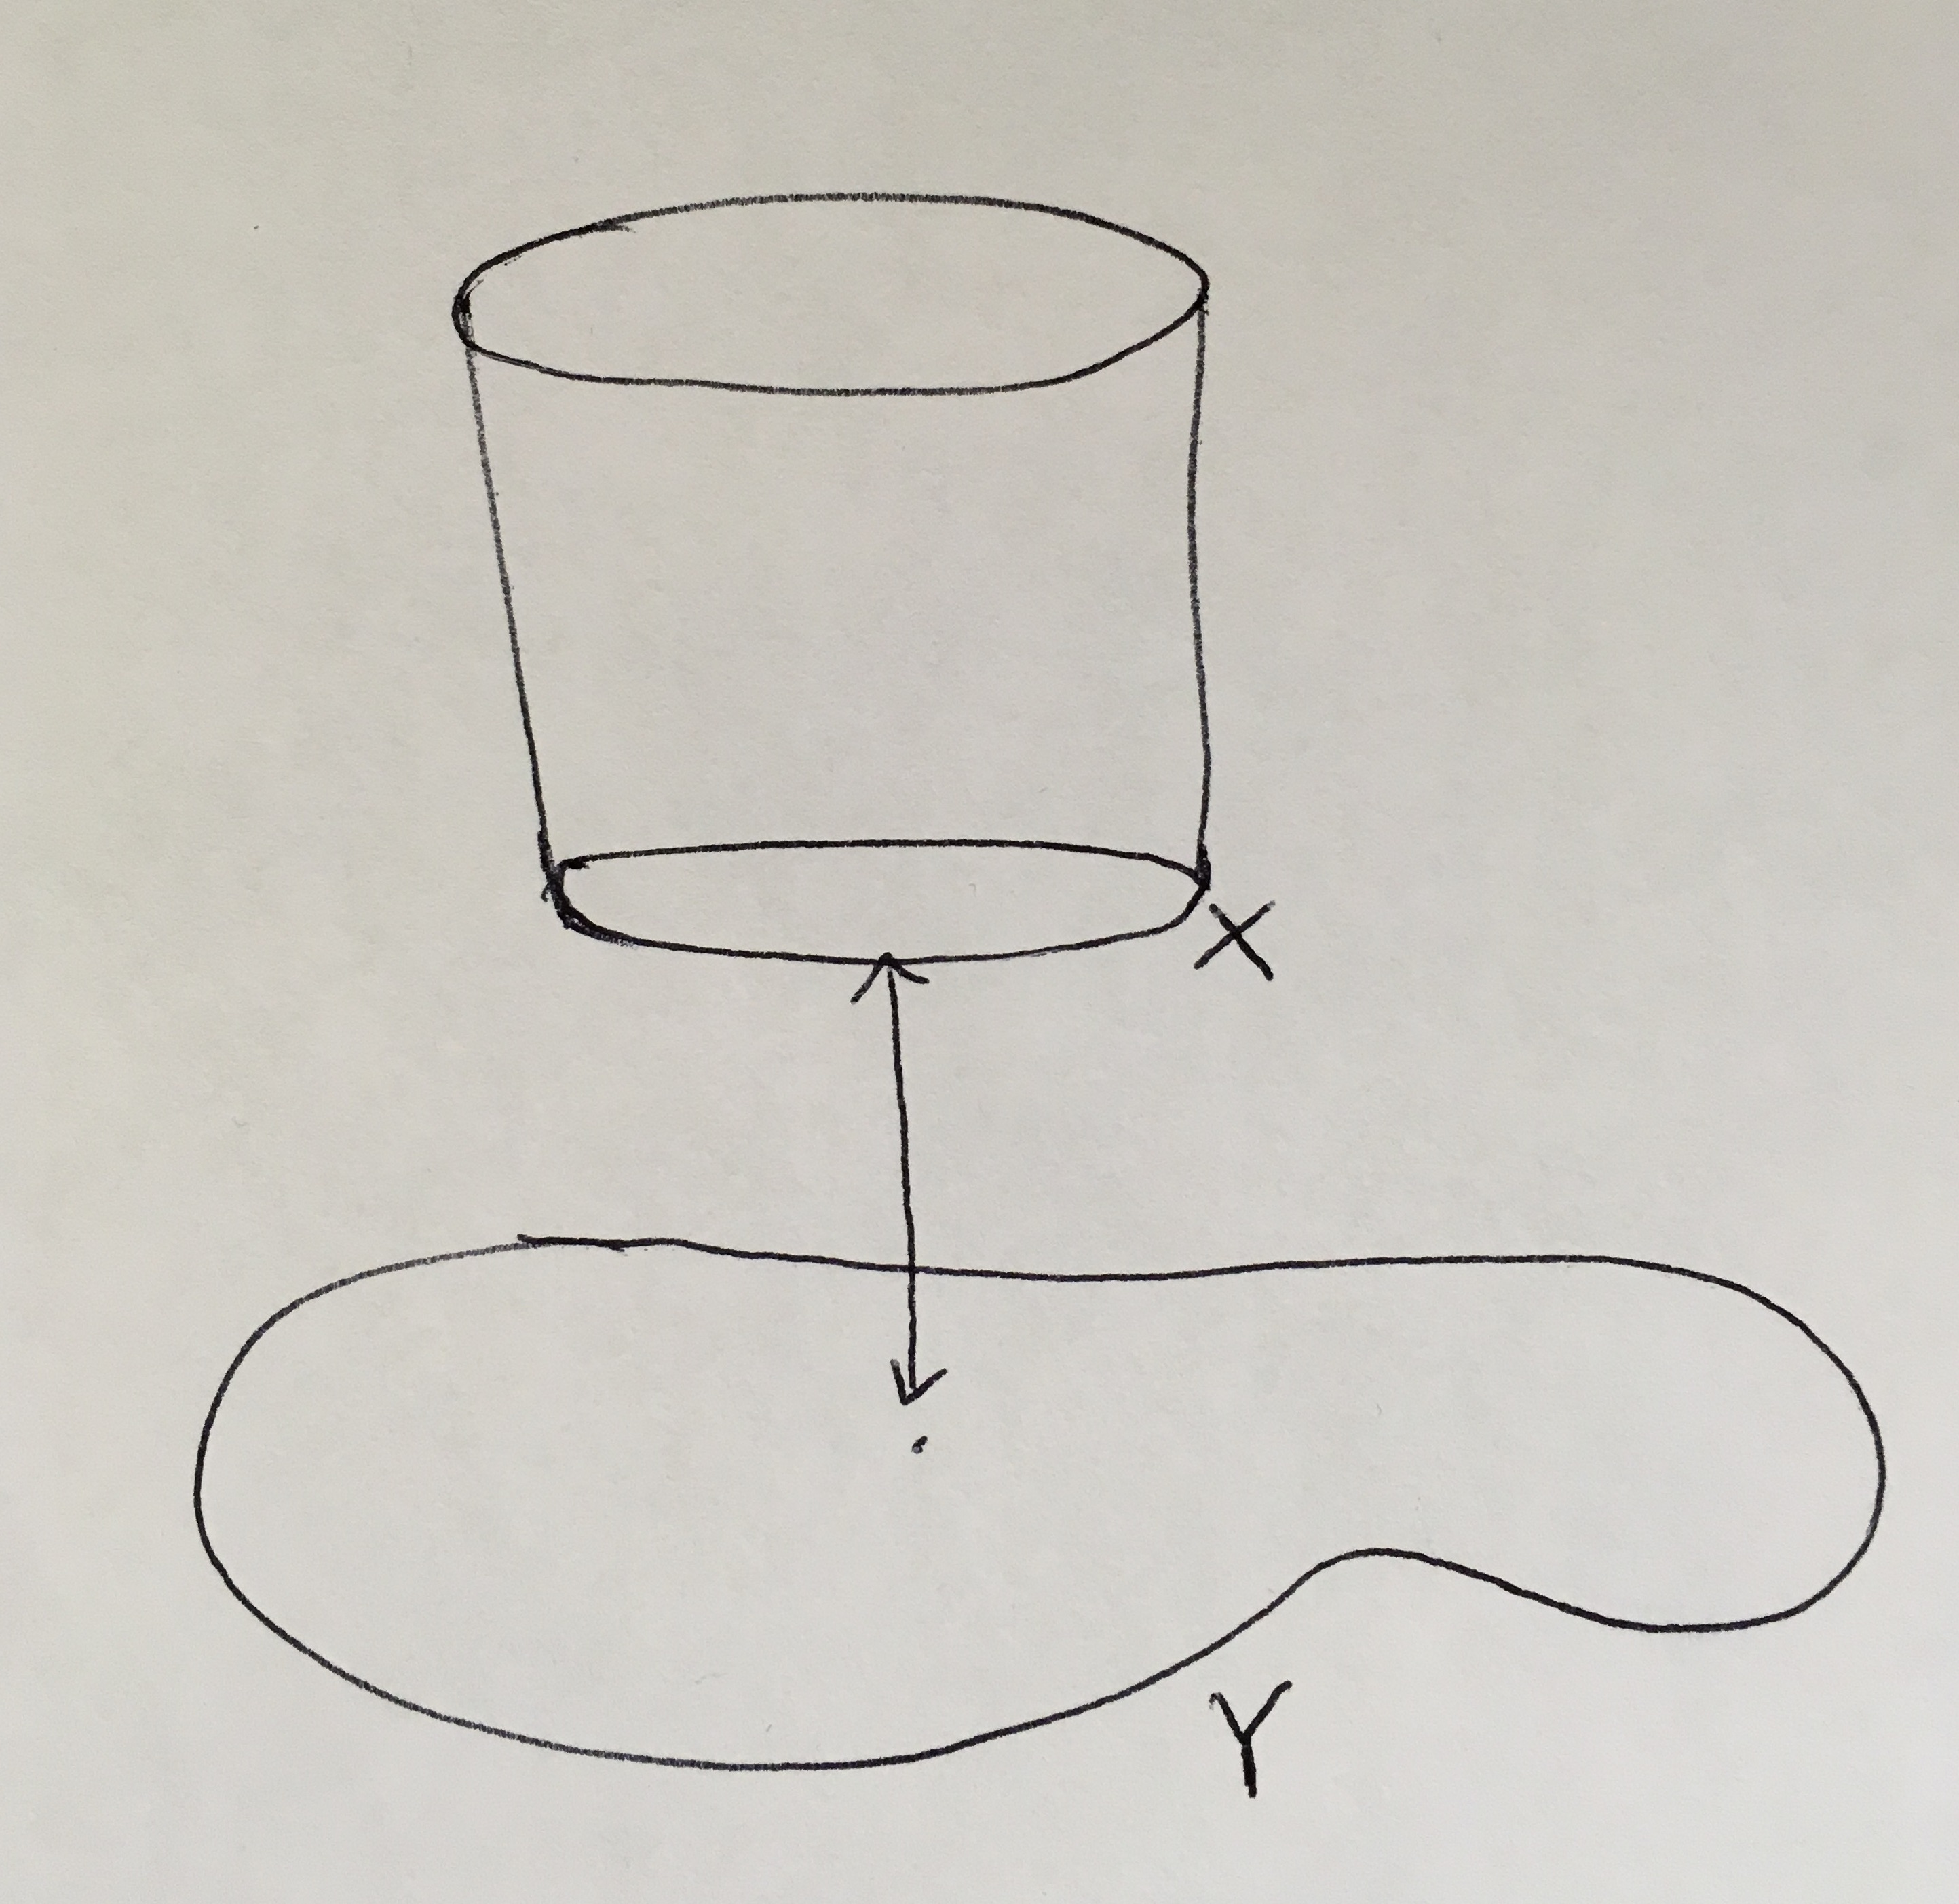
\includegraphics[width=30mm]{map-cyl.jpg}
\end{figure}

This is precisely the pushout of the span $X \times I \overset{\sigma_0}{\longleftarrow} X \overset{g}{\longrightarrow} Y$. As it turns out, $g$ factors as
\[
\begin{tikzcd}
X \arrow[rr, "g", bend left] \arrow[r, "\iota"', hook] & \cyl(g) \arrow[r, "h"'] & Y
\end{tikzcd}
\] for some deformation retraction $h$. Further, $\iota$ is a cofibration, the dual notion to a fibration.
\end{remark}

\smallskip

Consider the subspace of $\Omega{S^n}$ consisting of all great circles passing through, say, the north pole. This is clearly homeomorphic to $S^{n-1}$. Thus, we get a LES in homology
\[
\begin{tikzcd}
\cdots \arrow[r] & \overbrace{H_{2n-2}(S^{n-1})}^{0} \arrow[r]  & \overbrace{H_{2n-2}(\Omega{S^n})}^{\Z} \arrow[r, "\cong"] & {H_{2n-2}(\Omega{S^n}, S^{n-1})} \arrow[lld] &                                                 \\
                 & \underbrace{H_{2n-3}(S^{n-1})}_{0} \arrow[r] & H_{2n-3}(\Omega{S^n}) \arrow[r, "\cong"]                  & {H_{2n-3}(\Omega{S^n}, S^{n-1})} \arrow[r]   & \cdots \arrow[lld]                              \\
                 &                                              & \underbrace{H_{n+1}(S^{n-1})}_{0} \arrow[r]               & H_{n+1}(\Omega{S^n}) \arrow[r, "\cong"]      & {H_{n+1}(\Omega{S^n}, S^{n-1})} \arrow[lld]     \\
                 &                                              & \underbrace{H_{n}(S^{n-1})}_{0} \arrow[r]                 & H_{n}(\Omega{S^n}) \arrow[r, "\cong"]        & {H_{n}(\Omega{S^n}, S^{n-1})} \arrow[lld, "0"'] \\
                 &                                              & H_{n-1}(S^{n-1}) \arrow[r, "\overset{\cong}{f_{\ast}}"']  & H_{n-1}(\Omega{S^n}) \arrow[r, "0"']         & {H_{n-1}(\Omega{S^n}, S^{n-1})} \arrow[ld]      \\
                 &                                              &                                                           & \underbrace{H_{n-2}(S^{n-1})}_{0} \arrow[r]  & \cdots                                         
\end{tikzcd}.
\]

From this, we deduce that
\[
H_i(\Omega{S^n}, S^{n-1}) = \begin{cases} 0 & i \leq 2n-3
\\ \Z & i = 2n-2
\end{cases}.
\] By \cref{Hcor}(2), this means that
\[
\pi_i(\Omega{S^n}, S^{n-1}) = \begin{cases} 0 & i \leq 2n-3
\\ \Z & i = 2n-2
\end{cases}.
\]
This yields a LES in homotopy
\[
\begin{tikzcd}
\cdots \arrow[r] & \pi_{2n-2}(\Omega{S^n}) \arrow[r] & {\pi_{2n-2}(\Omega{S^n}, S^{n-1})} \arrow[ld] &                                                                  &                                                               &        \\
                 & \pi_{2n-3}(S^{n-1}) \arrow[r]     & \pi_{2n-3}(\Omega{S^n}) \arrow[r]             & {\overbrace{\pi_{2n-3}(\Omega{S^n}, S^{n-1})}^{0}} \arrow[ld]    &                                                               &        \\
                 &                                   & \pi_{2n-4}(S^{n-1}) \arrow[r, "\cong"]        & \underbrace{\pi_{2n-4}(\Omega{S^n})}_{\pi_{2n-3}(S^n)} \arrow[r] & {\underbrace{\pi_{2n-4}(\Omega{S^n}, S^{n-1})}_{0}} \arrow[r] & \cdots
\end{tikzcd},
\] which proves the following statement.

\begin{theorem}[Suspension]\label{ST}
If $0\leq i\leq 2n-4$, then $\pi_i(S^{n-1}) \cong \pi_{i+1}(S^n)$.
\end{theorem}

This can be generalized as follows.

\smallskip

\begin{exercise}[Freudenthal suspension]
Let $i \in \Z_{\geq 1}$ and suppose that the space $X$ satisfies $\pi_n(X) =0$ for each $0\leq n \leq i-1$. Show that $$\pi_i(X) \cong \pi_{i+1}(S{X})$$ through around dimension $2i-3$ (figure this out exactly), where $S({-})$ denotes the suspension functor.
\end{exercise}
\begin{proof}
We could use a spectral sequence argument together with the relative Hurewicz theorem. Rather, let us show that it follows from the following famous theorem in homotopy theory:
\begin{theorem}[Blakers-Massey]\label{BM}
Suppose that 
\[
\begin{tikzcd}
X \arrow[d, hook] \arrow[r, hook] & B \arrow[d] \\
A \arrow[r]                        & C          
\end{tikzcd}
\] is a pushout diagram. Also, suppose that $\pi_n(B, X)=0$ and $\pi_m(A, X)=0$ for each $0\leq n \leq k_1$ and each $0\leq m \leq k_2$. The map $\left(A, X\right) \to \left(C, B\right)$ of pairs induces an isomorphism $\pi_n(A, X) \overset{\cong}{\longrightarrow} \pi_n(C, B)$ for each $0 \leq n \leq k_1 + k_2 -1$.
\end{theorem}
Now, let us prove the Freudenthal suspension theorem with an upper bound of $2i-2$ rather than $2i-3$. To start, decompose $S{X}$ into the union of two cones $\underset{\text{top}}{C_+{X}}$ and $\underset{\text{bottom}}{C_{-}{X}}$ that meet at a copy of $X$. Note that $S{X}$ is precisely the pushout of the diagram
\[
\begin{tikzcd}
C_{-}{X} & X \arrow[l, hook'] \arrow[r, hook] & C_{+}{X}.
\end{tikzcd}
\]
As $C^+{X}$ is contractible, the LES of homotopy groups for the pair  $\left(C_{+}{X},X\right)$ shows that the map $\partial : \pi_{n+1}(C_{+}{X}, X) \to \pi_n(X)$ is an isomorphism. Similarly, we see that the map $\iota : \pi_{n+1}(S{X}) \to \pi_{n+1}(S{X}, C_{-}{X})$ induced by inclusion is an isomorphism.  Consider the sequence of homomorphisms
\[
\begin{tikzcd}
\pi_n(X) \arrow[r, "\partial^{-1}"] & {\pi_{n+1}(C_{+}{X},X)} \arrow[r, "\psi"] & {\pi_{n+1}(S{X}, C_{-}{X})} \arrow[r, "\iota^{-1}"] & \pi_{n+1}(S{X})
\end{tikzcd}
\]
where $\psi$ is induced by pullback. Since $\pi_n(X) =0$ for each $0\leq n \leq i-1$, the LES for the pair $\left(C_{\pm}{X}, X\right)$ also  shows that $\pi_n(C_{\pm}{X}) =0$ for any $0 \leq n \leq i$. By \cref{BM}, it follows that $\psi$ is an isomorphism so long as $n+1 \leq 2i-1$. Hence $\pi_n(X) \cong \pi_{n+1}(S{X})$ for any $n \leq 2i-2$, as desired.

\medskip


Furthermore, the upper bound of $2i-2$ is sharp. Indeed, we have that
\bi
\item $\pi_0(S^2) = \pi_1(S^2) =0$,
\item $\pi_3(S^2) \cong \Z$, and
\item $\pi_4(S^3) \cong \Z/2$.
\ei
If we could increase our upper bound to $2i-1$, then we would have an isomorphism  $\pi_3(S^2) \cong  \pi_4(S^3)$, which is impossible.
\end{proof}

\subsection{Lecture 13}

As expected, spectral sequences have exact analogues in cohomology.  Before introducing them, let us review a bit of singular cohomology theory.  Let $X$ be a cell complex and let $n\in \Z_{\geq0}$. Recall that $C_n(X)$ the free abelian group on the set of all $n$-cells of $X$ and the boundary map $\partial_n : C_n(X) \to C_{n-1}(X)$. Let $$C^{n}(X) = \Hom(C_{n}(X), \Z) $$ and define the homomorphism $\delta^n : C^n(X) \to C^{n+1}(X)$ by $$\delta^n(\varphi) = \varphi \circ \partial_n.$$

\begin{theorem}\label{cohomiso}
$H^n(X;\Z) \cong \frac{\ker{\delta^{n+1}}}{\im{\delta^n}}$.
\end{theorem}

\begin{exmp}
$H^{\ast}(\CP^n; \Z) \cong \faktor{\Z[x]}{\left(x^{n+1}\right)}$ with $\underset{\text{dim.}}{\left\lvert{x}\right\rvert} =2$.
\end{exmp}

\begin{theorem}[Poincar\'e duality]
If $M$ is a connected orientable $n$-manifold, then $H_i(M) \cong H^{n-i}(M)$.
\end{theorem}

\medskip

Now, a cohomological spectral sequence consists of the following data: 
\bi
\item for each $r\in \Z_{\geq 0}$, a family of abelian groups $\left\{E_r^{p,q}\right\}_{p,q\in \Z}$ and
\item a family of maps  $\left\{d_r^{p,q} : E_r^{p,q} \to E_r^{p+r, q-r+1}\right\}_{p,q\in \Z}$ (called \textit{differentials})  such that
\item $d_r^{p,q} \circ d_r^{p-r, q+r-1} =0$ and
\item $E_{r+1}^{p,q} = \frac{\ker{d_r^{p,q}}}{\im{d_r^{p-r, q+r-1}}}$.
\ei

Again, we shall consider only \textit{first-quadrant} spectral sequences, i.e., those for which $E^{p,q}_r =0$ unless $p,q\geq 0$.
As a result, there is some $k\in \N$ such that $E_r = E_{r+1}$ for any $r\geq k$. 

\begin{notation}
$E_{\infty} \coloneqq E_k$.
\end{notation}

\begin{defn}[Convergence]
 We say that a spectral sequence $E_{\ast} \coloneqq \left(E_r, d_r\right)$ \textit{converges} to a sequence of abelian groups $\left\{D^n\right\}_{n \in \Z_{\geq 0}}$, written as 
 \[
E_{\ast} \Rrightarrow \left\{D^n\right\},
 \]
 if for each $n$, there exists a filtration
 \[
 \cdots \subset D^{n+1, {-1}} = \left\{0\right\} \subset D^{n,0} \subset \cdots \subset D^{1,n-1} \subset D^{0,n} =D^n
 \]
 of $D^n$ such that $\frac{D^{p,q}}{D^{p+1, q-1}} \cong E_{\infty}^{p,q}$.
\end{defn}

\begin{theorem}\label{spfib}
Let $B$ be simply connected and path connected and suppose that $\pi: E \to B$ is a fibration with fiber $F$. There exists a (first-quadrant) spectral sequence $\left(E^r, d_r\right)$ that
\be[label=(\alph*)]
\item converges to $\left\{H^n(E)\right\}_{n\in \Z_{\geq 0}}$ and
\item satisfies $E^{p,q}_2 \cong H^p(B; H^q(F))$.
\ee
\end{theorem}

In pictures, we have

\begin{center}
\begin{sseqdata}[name = gen', cohomological Serre grading, no ticks]
\begin{scope}[background]
\node at (\xmax/2,\ymax+1.2) {\textup{Page \page}};
\node[font = \small] at (\xmax/2,-1.7) {H^p(B)\coloneqq H^p(B; H^0(F))};
\node at (-1.5,\ymax/2) {H^q(F)};
\end{scope}
\class(0,0)
\class(0,1)
\class(0,2)
\class(1,2)
\class(2,2)
\class(1,0)
\class(2,0)
\class(1,1)
\class(2,1)
\class(3,0)
\class(3,1)
\class(3,2)
\d2(0,2)
\end{sseqdata}
\printpage[ name = gen', page = 2 ]
\end{center}

\[
\begin{tikzcd}
H^q(E) \arrow[r, equals] \arrow[rrrrr, "i^{\ast}", bend right]   & {D^{0,q}} \arrow[r, two heads]   & {E_{\infty}^{0,q}} \arrow[r, hook] & \cdots \arrow[r, hook]      & {E_2^{0,q}} \arrow[r, equals]              & H^q(F) \\
                                                         &                                  &                                    &                             &                                    &        \\
                                                                                                                  &                                  &                                    &                             &                                    &        \\
H^p(B) \arrow[r, equals] \arrow[rrrrr, "\pi^{\ast}", bend right] & {E_2^{p,0}} \arrow[r, two heads] & {E_3^{p,0}} \arrow[r, two heads]   & \cdots \arrow[r, two heads] & {E_{\infty}^{p,0}} \arrow[r, hook] & H^p(E)
\end{tikzcd}.
\]

\bigskip

Let $X$ be a cell complex. Recall the \textit{cup product} operation $H^i(X) \times H^j(X) \overset{\smile }{\longrightarrow} H^{i+j}(X)$ on cohomology, which is both bilinear and \textit{anti-commutative} in the sense that
\[
x \smile y = \left({-1}\right)^{ij}y \smile x.
\]

Consider the constant map $C_0(X) \to \Z$ given by $D^0 \mapsto 1$, which corresponds to an element $\mathbf{1}$ of $H^0(X)$ via \cref{cohomiso}. We have that
\[
{-\mathbf{1}}\smile x = x \smile \mathbf{1} = \mathbf{1}.
\]

\smallskip

Suppose that $Y$ is another cell complex. Let $x \in H^i(X)$ and $y\in H^j(X)$ and let $f$ denote a map $Y \to X$. Then 
\[
f^{\ast}(x\smile y) =f^{\ast}(x)\smile f^{\ast}(y),
\] i.e., $f^{\ast}$ is a graded ring homomorphism. Now, $X \times Y$ carries a cell complex structure with $n$-cells of the form 
\[
D^i \times D^j, \  \quad i+j =n
\] and $n$-skeleton
\[
\left(X\times Y\right)^n \equiv \bigcup_{i+j =n}X^i \times Y^j.
\] We have that 
\[
C_n(X \times Y) \cong C_n(X) \otimes_{\Z} C_n(Y)
\] and, in light of the fact that $\partial(D^i \times D^j) = \left(\partial{D^i} \times D^j\right) \cup \left(D^i \times \partial{D^j}\right)$, that
\[
\partial[D^i \times D^j] = \partial[D^i] \otimes D^j + ({-1})^i[D^i]\otimes \partial[D^j].
\]
Consider any two maps $f: C_i(X) \to \Z$ and $g: C_j(X) \to \Z$, extending them both by $0$ to the entire graded abelian group $C_{\ast}(X)$. Define $f \otimes g : C_m(X \times Y)\cong C_m(X) \otimes C_m(Y) \to \Z$ by 
\[
\left(f \otimes g\right)\left(u \otimes v\right) = f(u) \cdot g(v).
\]


\begin{prop}
$\delta(f \otimes g) = \delta{f} \otimes g + (-1)^i{f} \otimes \delta{g}$.
\end{prop}

As it turns out, this means that the map $\left(f,g\right) \mapsto \left(f \otimes g\right)$ induces an operation $H^i(X) \times H^j(Y) \overset{\times}{\longrightarrow} H^{i+j}(X\times Y)$ on cohomology known as the \textit{cross product}. The relation between the cup and cross product has the form $\Delta^{\ast}(x\times y) = x\smile y$, where $\Delta : X \to X \times X$ denotes the diagonal map.

\medskip

In general, let $R_1$, $R_2$, and $R_3$ be commutative rings and let $\mu : R_1 \times R_2 \to R_3$ denote  ``multiplication." This induces the cup product on cohomology
\begin{align*}
H^i(X; R_1)  \times H^j(X; R_2) &  \xrightarrow{\smile}H^{i+j}(X; R_3)
\\ &  \Downarrow \quad \quad \quad \quad
\\ H^p(B, H^q(F)) \times H^{p'}(B, H^{q'}(F)) &  \xrightarrow{\smile}H^{p+p'}(B, H^{q+q'}(F))
\\ E_2^{p,q} \times E_2^{p', q'} &   \xrightarrow{\smile}E_2^{p+p', q+q'}. 
\end{align*}

\begin{prop}
For any $r\in \Z_{\geq 2}$, there is a certain operation $\smile_r : E_r^{p,q} \times E_r^{p',q'} \to E_r^{p+p', q+q'}$ such that
\[
d_r(x\smile y) = d_r(x) \smile y + ({-1})^{p+q}x \smile d_r(y).
\] 
\end{prop}
\begin{proof}[Construction]
Let $r\in \Z_{\geq 2}$ and  suppose, for induction, that we have already constructed $\smile_r$. Let $x \in E_r^{p,q}$ and $y\in E_r^{p',q'}$. Suppose that $d_r{x} =d_r{y} =0$, so that $d_r(x \smile y) =0$. If $y = d_r(z)$, then 
\[
x \smile y = x \smile d_r(z) = d(x\smile z) \pm \underbrace{d_r(x)}_{0} \smile z.
\] by induction. This means that $\smile_r$ induces a pairing $\smile_{r+1}$ on $E_{r+1}$. To complete our induction on $r$, simply  take the ordinary cup product on cohomology to be $\smile_2$.
\end{proof}

Now, given the filtration
\[
\left\{0\right\} \subset D^{n,0} \subset \cdots \subset D^{0,n} \subset H^n(E),
\] the operation $\smile_r$ on $E_r$ carries $D^{p,q} \times D^{p',q'}$ to $D^{p+p', q+q'}$ where $p+q = p'+q' =n$, thereby inducing a pairing $$\smile_{\infty}: E_{\infty}^{p,q} \times E_{\infty}^{p',q'} \to E_{\infty}^{p+p', q+q'}$$
on $E_{\infty}$.

\smallskip

\begin{exmp}
Consider the fiber bundle $S^1 \to S^{2n+1} \twoheadrightarrow \CP^n$, so that
\[
E_2^{p,q} \cong H^p(\CP^n; H^q(S^1)).
\] Pick a generator $x$ of  the group $H^1(S^1) \cong \Z$. Then the cohomology ring $H^{\ast}(S^1)$ is isomorphic to $\faktor{\Z[x]}{\left(x^2\right)}$, and 
\[
H^i(S^1) \cong \begin{cases} \Z & i =0,1 \\ 0 & i>1 \end{cases}.
\] Moreover, recall that
\[
H^i(\CP^n) \cong \begin{cases}  
\Z & 0\leq i \leq 2n, \ i \equiv 0 \mod 2
\\ 0 & \text{otherwise}
\end{cases},
\]
which yields
\[
\begin{sseqpage}[ cohomological Serre grading,  classes = {draw = none}, y tick gap = 2.0 em, scale = 1.6, y axis gap = 40pt, x axis extend end = 1.1cm, x range = {0}{6}, y range = {0}{2},
x tick handler = {
\ifnum#1 = 0\relax
0
\else
\ifnum#1 = 1\relax
1
\else	
\ifnum#1 = 2\relax
2
\else	
\ifnum#1 = 3\relax
3
\else	
\ifnum#1 = 4\relax
4
\else	
\ifnum#1 = 5\relax
{\cdots}
\else	
\ifnum#1 = 6\relax
% \vphantom is fragile so we \protect it
\protect\vphantom{2}2n
\else
#1n
\fi
\fi
\fi
\fi
\fi
\fi
\fi
}]
\begin{scope}[background]
\node at (\xmax/2,\ymax+0.6) {\textup{Page 2}};
\node[font = \small] at (\xmax/2,-1.1) {H^p(\CP^n)};
\node at (-2.0,\ymax/2) {H^q(S^1)};
\end{scope}
\class["\Z"](0,0)
\class["\Z"](0,1)
\class(0,2)
\class(0,3)
\class["\Z"](2,0)
\class[circle, fill](2,1)
\class(1,0)
\class(1,1)
\class(2,2)
\class(2,3)
\class(3,-1)
\class["\Z"](4,0)
\class["\Z"](6,0)
\d["d_2"]2(0,1)
\d["d_2"]2(2,1)
\end{sseqpage}
\]
where each $d_2$ is an isomorphism. Suppose that $x$ is a generator of $H^1(S^1)$ and let $c = d_2(x)$. Then $$d_2(c \smile x) = c\smile d_2(x) = c^2,$$ which is a generator of $H^4(\CP^n)$. Similarly, $c^i$ is a generator of $H^{2i}(\CP^n)$ for each $i\in \Z_{\geq 0}$.
\end{exmp}

By letting $c^0 =1$ and making $n$ large enough, we have determined the ring structure of $H^{\ast}(\CP^{\infty})$.

\begin{theorem}\label{chbase}
If $c_1$ is a generator of $H^2(\CP^{\infty})\cong \Z$, then $\underbrace{H^{\ast}(B_{S^1})  =H^{\ast}(\CP^{\infty})}_{\cref{classcirc}} \cong \Z[c_1]$.
\end{theorem}

\section{Characteristic classes}

\subsection{Lecture 14}

Recall the space $B_{\Un(n)} = B_{\GL(n, \C)}$ of $n$-planes in $\C^{\infty}$ as well as the space $B_{\Or(n)} = B_{\GL(n, \R)}$ of $n$-planes in $\R^{\infty}$. We want to classify the graded rings 
$H^{\ast}(B_{\Un(n)}; \Z)$ and  
$H^{\ast}(B_{\Or(n)}; \Z_2)$. Let's begin with the former.

\medskip

Consider the embedding $\Un(n-1) \hookrightarrow \Un(n)$ given by $A \mapsto \begin{bmatrix} A & 0 \\ 0 & 1\end{bmatrix}$. Consider also the mapping $\Un(n) \to S^{2n-1}$ given by $A \mapsto A{e_n}$. These fit into a ``short exact sequence"
\[
\label{eqn:ses} 0 \to \Un(n-1)\to \Un(n) \to S^{2n-1} \to 0 \tag{1}
\] of spaces,
and thus the bundle
\[\label{eqn:Bfib}
 \frac{\Un(n)}{\Un(n-1)} \to B{\Un(n-1)} \overset{\pi}{\longrightarrow} B{\Un(n)} \tag{2}
\] has fiber $S^{2n-1}$.

\begin{remark}
Let us make \eqref{eqn:ses} precise. Note that $\Un(n)$ acts transitively on $S^{2n-1}$ because any point in $S^{2n-1}$ belongs to at least one orthonormal bases of $\C^n$.This means that $S^{2n-1}$ is a \textit{homogenous} $\Un(n)$-space. 
\begin{prop}
Any homogenous $G$-space $X$ is homeomorphic to the coset space $\faktor{G}{\stab_G(\vec{o})}$ where $\vec{o}$ is any choice of ``identity." 
\end{prop}
In our case, let $\vec{o} = e_n$, so that $\stab_{\Un(n)}(\vec{o}) = \Un(n-1)$. 
\end{remark}

\medskip

Now, \eqref{eqn:Bfib} induces a spectral sequence $E_{\ast}$ converging to $H^{\ast}(B{\Un(n-1)})$ such that
\[
E_2^{p,q} = H^p(B{\Un(n)}; H^q(S^{2n-1}))
\]
and 
\[
\begin{tikzcd}
H^p(B{\Un(n)}) \arrow[r] \arrow[rrrrr, "\pi^{\ast}", bend right] & {E_2^{p,0}} \arrow[r, two heads] & {E_3^{p,0}} \arrow[r, two heads] & \cdots \arrow[r, two heads] & {E_{\infty}^{p,0}} \arrow[r, hook] & H^p(B{\Un(n-1)})
\end{tikzcd}
\] commutes. If $p< 2n$, then $H^p(B{\Un(n)}) \cong E_{\infty}^{p,0}$, in which case $\pi^{\ast}$ is injective. Also, we have that $E_2^{p-k, k} = E_{\infty}^{p-k, k}$ whenever $0<p-k < 2n+1$, so that $\pi^{\ast}$ is surjective whenever $p<2n$. It follows that $\pi^{\ast}$ is an isomorphism 
\[
\label{eqn:Biso} H^p(B{\Un(n)}) \cong H^p(B{\Un(n-1)}) \tag{3}
\] when $p\leq 2n-1$.

\smallskip

Consider the differential $d_2 : \underbrace{H^{2n-1}(S^{2n-1})}_{\Z} \to H^{2n}(B{\Un(n)})$ and pick a generator $g_n$ of $H^{2n-1}(S^{2n-1})$, i.e., an orientation of $S^{2n-1}$. Let
\[
c_n= d_{2}(g_n).
\]
In light of \eqref{eqn:Biso}, we see that
\[
c_i \in H^{2i}(B{\Un(n)}) \cong \cdots \cong H^{2i}(B{\Un(i+1)}) \cong H^{2i}(B{\Un(i)}) 
\] for each $i\leq n$. Abusing notation, we shall write $c_i \in H^{2i}(B{\Un(i)})$.
\medskip

\begin{theorem}\label{cherngens}
$H^{\ast}(B{\Un(n)}; \Z)\cong  \Z[c_1, \ldots, c_n]$
\end{theorem}
\begin{proof}
Proceed by induction on $n\in \N$. Our base case holds by virtue of \cref{chbase}. Assume that 
\[
H^{\ast}(B{\Un(n-1)}) \cong \Z[c_1, \ldots, c_{n-1}].
\]
Note that $E_{2n}=E_{\infty}$ and $E_{2n-1}=E_2$, yielding
\[
\begin{sseqpage}[ cohomological Serre grading,  classes = {draw = none}, y tick gap = 2.0 em, scale = 1.6, y axis gap = 20pt, x axis extend end = 1.1cm, x range = {0}{6}, y range = {0}{2},
x tick handler = {
\ifnum#1 = 0\relax
0
\else
\ifnum#1 = 1\relax
1
\else	
\ifnum#1 = 2\relax
2
\else	
\ifnum#1 = 3\relax
3
\else	
\ifnum#1 = 4\relax
4
\else	
\ifnum#1 = 5\relax
{\cdots}
\else	
\ifnum#1 = 6\relax
% \vphantom is fragile so we \protect it
\protect\vphantom{2}2n
\else
#1n
\fi
\fi
\fi
\fi
\fi
\fi
\fi
}, 
y tick handler = {
\ifnum#1 = 0\relax
0
\else
\ifnum#1 = 1\relax
% \vphantom is fragile so we \protect it
{\vdots}
\else
2n-1
\fi
\fi
}]
\begin{scope}[background]
\node at (\xmax/2,\ymax+0.6) {\textup{Page $2n-1$}};
\node[font = \small] at (\xmax/2,-1.1) {H^p(B{\Un(n)})};
\node at (-2.0,\ymax/2) {H^q(S^{2n-1})};
\end{scope}
\class["\Z"](0,0)
\class(0,1)
\class["g_n"](0,2)
\class(0,3)
\class["c_1"](2,0)
\class(2,1)
\class["0"](1,0)
\class["0"](3,0)
\class(1,1)
\class(2,2)
\class(2,3)
\class(3,-1)
\class(0, 3)
\class["\cdots"](5,0)
\class["c_2"](4,0)
\class["c_{n}"](6,0)
\draw[->](0,2) to["d_{2n-1}"] (6,0);
\end{sseqpage}.
\]
{??}
\end{proof} 

\smallskip

We call $c_i$ the $i$-th \textit{Chern class} of $B{\Un(n)}$. The following may be seen as a real analogue to \cref{cherngens}.

\begin{theorem}
$H^{\ast}(B{\Or(n)}, \Z_2) \cong \Z\left[w_1, \ldots, w_n\right]$ for certain cohomology classes $w_i \in H^i(B{\Or(n)}, \Z_2)$.
\end{theorem}

We call $w_i$ the $i$-th \textit{Stiefel-Whitney} class of $B{\Or(n)}$.


\begin{exmp}
Let $M$ be a smooth $n$-manifold. Consider the tangent bundle $T{M}$ with group $\Or(n)$ and fiber $\R^n$. Let $f : M \to B{\Or(n)}$ denote the classifying map for $T{M} \overset{\pi}{\longrightarrow} M$, so that  $f^{\ast}{\gamma_n} = \pi$ where $\gamma_n$ denotes the universal $\Or(n)$-bundle. For each $i\in \left\{1, 2, \ldots, n\right\}$, the $i$-th Stiefel-Whitney class for $M$ is exactly the element 
\[
w_i(M) \equiv f^{\ast}{w_i\left(E_{\Or(n)}\right)}
\] of $H^i(M, \Z_2)$. Note that $w_i$ is natural in the sense that  
$w_i\left(f^{\ast}{E_{\Or(n)}}\right) =  f^{\ast}{w_i\left(E_{\Or(n)}\right)}$.  Now, the complexification of $\pi$ is the vector bundle $T_{\C}{M}$, with classifying map $f: M \to B{\Un(n)}$. In this case, the
$i$-th Chern class for $M$ is exactly the element
\[
c_i(M) \equiv f^{\ast}{c_i\left(E_{\Un(n)}\right)}
\] of $H^{2i}(M, \Z)$.
 In general, any  vector bundle $\xi$ with group $\Or(n) \subset \Un(n)$ and fiber $\R^n$ has a complexification $\xi \otimes \C$ with group $\Un(n)$ and fiber $\C^n$. Every fiber $E_x$ of $\xi$ is converted to a fiber $E_x \oplus E_x$ of $\xi \otimes \C$ with scalar multiplication given by $i \cdot \left(x,y\right) \equiv \left({-y}, x\right)$. The \textit{$i$-th Pontryagin class} for $M$ is exactly
\[
p_i(M) \equiv \left({-1}\right)^ic_{2i}(T{M} \otimes \C).
\]
\end{exmp}

\medskip

For any two complex vector bundles $\xi$ and $ \eta$ over $X$ with groups $\Un(n)$ and $\Un(m)$, respectively, we can form a new vector bundle $\xi \oplus \eta$ with group $\Un(n +m)$ and fiber $\C^n \times \C^m$ such that
\[
h_{\alpha{\beta}}(\xi \oplus \eta) \equiv \begin{bmatrix}  h_{\alpha{\beta}}(\xi) & 0 \\ 0 & h_{\alpha{\beta}}(\eta) \end{bmatrix}.
\]

\begin{term} 
The sum $c(\xi) \coloneqq 1 + c_1 + c_2 + \cdots + c_n \in H^{\ast}(X, \Z)$ is called the \textit{total Chern class} for $\eta$. If $\xi$ is instead a real vector bundle, then we have the \textit{total Stiefel-Whitney class} $w(\xi) \coloneqq 1 + w_1 + w_2 + \cdots + w_n \in H^{\ast}(X, \Z_2)$.
\end{term}

\begin{theorem}[Whitney sum formulas] $ $
\be
\item $c(\xi \oplus \eta) = c(\xi) \smile c(\eta)$, i.e.,  $c_k(\xi \oplus \eta) = \sum_{i+j =k}c_i(\xi) \smile c_j(\eta), \  \ c_0 \equiv 1$.
\item $w(\xi \oplus \eta) = w(\xi) \smile c(\eta)$, i.e.,  $w_k(\xi \oplus \eta) = \sum_{i+j =k}w_i(\xi) \smile w_j(\eta), \ \ w_0 \equiv 1$.
\ee
\end{theorem}


\begin{exercise}
Let $\xi$ and $\eta$ be fiber bundles over a CW complex $X$ with group $U(1)\cong S^1$ and fiber $\C$, i.e., (complex) line bundles over $X$. Consider the tensor bundle $\xi \otimes \eta$. 
\be[label=(\alph*)]
\item Show that the set $\lb(X)$ of isomorphism classes of line bundles over $X$ is an abelian group under $\otimes$. 
\item Compute $c_1(\xi \otimes \eta)$ where $c_1$ denotes the first Chern class.
\ee
\end{exercise}
\begin{proof} $ $
\be[label=(\alph*)]
\item It is easy to see that $\otimes$ is commutative and associative. It is also easy to see that the natural isomorphism $\C \otimes \C \cong \C$ extends to an isomorphism between $\xi \otimes \eta$ and the trivial line bundle $X \times \C$, which is thus the identity element of $\lb(X)$. 

\smallskip

It remains to show that $\lb(X)$ has all inverses. To this end, consider the conjugate line bundle $\bar{\xi}$. If $h_{\beta{\alpha}}: U_{\alpha} \cap U_{\beta} \to S^1$ is any transition function for $\xi$, then the corresponding transition function for $\xi \otimes \bar{\xi}$ is given by 
\[
\tilde{h}_{\beta{\alpha}} \coloneqq h_{\beta{\alpha}} \otimes \overline{h_{\beta{\alpha}}} : U_{\alpha} \cap U_{\beta} \to S^1, \ \quad x \mapsto h_{\beta{\alpha}}(x)\cdot \overline{h_{\beta{\alpha}}(x)}.
\] But this means that every transition function for $\xi \otimes \bar{\xi}$ is the constant map at $1$. As a result,
\[
\label{eqn:iso} \tilde{h}_{\beta} \circ \tilde{h}_{\alpha}^{-1}(x, f)=\left(x, f\right), \tag{$\star$}
\] i.e., the local trivializations $\tilde{h}_{\alpha}$ and $\tilde{h}_{\beta}$ for $\xi \otimes \bar{\xi}$ agree on $U_{\alpha} \cap U_{\beta}$.  By gluing together these local trivializations, we get a well-defined bundle isomorphism $$\tilde{h} \equiv \bigcup_{\alpha}h_{\alpha} : \xi \otimes \bar{\xi} \overset{\cong}{\longrightarrow} X \times \C.$$ This proves that $\bar{\xi}$ is the inverse of $\xi$.
\item Since $U(1)$ is a topological group, we can apply the Milton construction to it to obtain the universal bundle $$p_{U(1)} : L \to B{U(1)} = \CP^{\infty}.$$ For each $i\in \left\{1,2\right\}$, let $\pi_i:  \CP^{\infty}\times  \CP^{\infty} \to  \CP^{\infty}$ denote the $i$-th projection. Consider now the tensor bundle 
\[
\tilde{L} \coloneqq \underbrace{\pi_1^{\ast}(L)}_{L_1} \otimes \underbrace{\pi_2^{\ast}(L)}_{L_2}
\]
over $\CP^{\infty}\times  \CP^{\infty}$. Then $c_1(\tilde{L})$ belongs to $H\coloneqq H^2(\CP^n \times \CP^n; \Z)$. From lecture, we know that $H^{\ast}(\CP^{\infty}; \Z)$ is precisely the infinite cyclic group generated by $c_1(L)$. In particular, it is a finitely-generated abelian group. Further, $ \CP^{\infty}$ is a CW complex as the colimit of CW complexes. Since $H^0(\CP^{\infty}; \Z) = \Z$ and $H^1(\CP^{\infty}; \Z) =0$, it follows from the K\"unneth theorem  that 
\[
\label{eqn:2}   
H \cong  \left(H^2(\CP^{\infty}; \Z) \otimes \Z\right) \oplus \left(\Z \otimes H^2(\CP^{\infty}; \Z)\right)\cong H^2(\CP^{\infty}; \Z) \oplus H^2(\CP^{\infty}; \Z) . \tag{1}
\]  
Under this sequence of isomorphisms, $c_1(\tilde{L})\in H$ corresponds uniquely to $\left(nc_1(L), mc_1(L)\right)$ for some $n,m \in \Z$. Choose any point $P\in \CP^{\infty}$ and let $i : \left\{P\right\} \times \CP^{\infty} \hookrightarrow \CP^{\infty} \times \CP^{\infty}$ denote the inclusion map. Taking the pullback of $L$ along $i$ yields a line bundle $i^{\ast}{L}$ over $\left\{P\right\} \times \CP^{\infty} \cong \CP^{\infty}$ that is isomorphic to $L_2$ viewed over $\CP^{\infty}$. Hence $c_1(i^{\ast}{L}) = c_1(L)$. But $i^{\ast}(c_1(L)) = mc_1(L)$, so that $c_1(L)= mc_1(L)$ by naturality of $c_1$. It follows that $m=1$. Similarly, we see that $n=1$. 

\smallskip

By inspection,  $c_1(L_1) + c_1(L_2)$ also corresponds uniquely to $\left(c_1(L), c_1(L)\right)$ under \eqref{eqn:2}. This means that 
\[
\label{eqn:3} c_1(L_1) + c_1(L_2) = c_1(\tilde{L}).  \tag{2}
\]
%Moreover, $\tilde{L}$ is isomorphic to $L_1$ when viewed over $\CP^{\infty} \times \left\{x_1\right\} \cong \CP^{\infty} $ and to $L_2$ when viewed over   $\CP^{\infty} \times \left\{x_2\right\} \cong \CP^{\infty} $ where  $x_1$ and $x_2$ are any two chosen elements of $\CP^{\infty}$. Denote these two new line bundles over $ \CP^{\infty} $ by $Q$ and $Q'$, respectively.  Then $\left(c_1(Q), c_1(Q')\right)$ equals $\left(c_1(L), c_1(L)\right)$ and thus corresponds uniquely to   $c_1(L_1) + c_1(L_2)$ via $\eqref{eqn:2}$. But it also corresponds uniquely to $c_1(\tilde{L})$, so that 

From \eqref{eqn:3}, we can derive that $c_1(\xi \otimes \eta) = c_1(\xi)+ c_1(\eta)$. Indeed, there must be maps $g_1, g_2 : X \to B{U(1)}$ such that $\xi \cong f_1^{\ast}{L}$ and $\eta \cong f_2^{\ast}{L}$. Note that the map $F\coloneqq \left(f_1, f_2\right) : X \to B{U(1)} \times B{U(1)}$ satisfies
\begin{align*}
F^{\ast}(L_1) & = F^{\ast}(\pi_1^{\ast}(L)) \cong \left(\pi_1 \circ F \right)^{\ast}(L) = f_1^{\ast}{L} \cong \xi
\label{eqn:4} \\ & \tag{3}
\\ F^{\ast}(L_2) & = F^{\ast}(\pi_2^{\ast}(L)) \cong \left(\pi_2 \circ F \right)^{\ast}(L) = f_2^{\ast}{L} \cong \eta.
\end{align*}
Now, recalling that for any line bundle $E$ over $X$, the local trivializations and transition functions of $F^{\ast}(E)$ are given by precomposition with $F$,  we easily see that
\[
\label{eqn:5} c_{1}(F^{*}(L_{1}) \otimes F^{*}(L_{2}))=c_{1}(F^{*}(L_{1} \otimes L_{2})). \tag{4}
\] Finally, by combining \eqref{eqn:3}, \eqref{eqn:4}, \eqref{eqn:5}, and the naturality of $c_1$, we get
\begin{align*}
c_1(\xi \otimes \eta) & = c_{1}(F^{*}(L_{1}) \otimes F^{*}(L_{2}))
\\ & =c_{1}(F^{*}(L_{1} \otimes L_{2}))
\\ & = F^{*}(c_1(L_{1} \otimes L_{2}))
\\ & = F^{*}(c_{1}(L_{1})+c_{1}(L_{2}))
\\ & =F^{*}(c_{1}(L_{1}))+F^{*}(c_{1}(L_{2}))
\\ & = c_{1}(F^{*}(L_{1}))+c_{1}(F^{*}(L_{2}))
\\ & = c_1(\xi) + c_1(\eta).
\end{align*}
\ee
\end{proof}

\end{document}
